\documentclass[3p,times]{article}

\usepackage[margin=0.7in]{geometry}

\usepackage{amssymb}
\usepackage{amsthm}
\usepackage{thmtools}
\usepackage{thm-restate}
\usepackage{hyperref}
\usepackage{amsmath}
\usepackage{cleveref}
\usepackage{algorithm2e}
\usepackage{graphicx}
\usepackage{subcaption}
\usepackage{xcolor}
\usepackage[version=4]{mhchem}
\newcommand{\N}{\mathbb{N}}
\newcommand{\R}{\mathbb{R}}
\newcommand{\I}{\mathcal{I}}
\DeclareMathOperator{\diag}{diag}
\declaretheorem[name=Theorem]{thm}
\declaretheorem[name=Lemma]{lemma}
\newtheorem{defn}{Definition}
\newtheorem{hypo}{H}
\usepackage[figuresright]{rotating}

\graphicspath{{Images/}}

\begin{document}

\title{Microbial interactions as drivers of a nitrification process in a chemostat}

\author{Pablo Ugalde-Salas, Héctor Ramírez C., Jérôme Harmand, Elie Desmond-Le Quéméner}
\date{}
\maketitle



\begin{abstract}
	This article deals with the inclusion of microbial ecology measurements such as abundances of operative taxonomic units in bioprocess modelling. The first part presents the mathematical analysis of a model that may be framed within the class of Lotka-Volterra models fitted to experimental data in a chemostat setting where a nitrification process was operated for over 500 days. The limitations and the insights of such an approach are discussed. In the second part,  the use of an optimal tracking technique (developed within the framework of control theory) for the integration of data from genetic sequencing in chemostat models is presented. The optimal tracking revisits the data used in the aforementioned chemostat setting. The method is able to reconstruct the different forms of nitrogen in the reactor by using the abundances of the operative taxonomic units, even though the synthesized control can not be guaranteed to be optimal. 
\end{abstract}



\section{Introduction}


Microbial communities and their interactions play a central role in the understanding of microbial ecosystems \cite{West2007}, and a current challenge is integrating genetic sequencing data in a deterministic modelling framework \cite{Widder2016,WADE201664}. Using the terminology from the thorough review in current methodologies on the deterministic modelling approaches of microbial community dynamics presented by Song \textit{et al.}\cite{Song2014}, this articles deals with population-based approaches where species are taken as the interacting units.

The classical ecological concept of species and niche in the microbial world is an elusive one: in the macro world one can clearly identify one species of another for reproductive reasons and their ability to give birth to offspring. In the case of bacteria and archea, reproduction goes simply by binary fission and exchange of some functional genes (the ability to synthesize or metabolize substances) can be acquired in evolutionary scale through lateral gene transfer \cite{Boucher2003}. Therefore as an ecological problem is hard to precise the 'niche' of 'microbial species'. These obstacles can be circumvented by considering the microbiologist concept of operative taxonomic unit (OTU) based on the clustering of organisms sharing similar sequences of 16S rDNA marker gene. In the past years considerable efforts have been made to measure the bacterial community composition. Tests such as fluorescence in situ hybridization, polymerase chain reaction (PCR) dependent techniques, and PCR independent techniques for the analysis of DNA have become a standard tool for studying  microbial diversity\cite{FERRERA2016790}. The contribution of this article is a new method to integrate the microbial community measurements in chemostat models, based on any sequencing or fingerprinting technique that can quantify the species abundances over time. In other words, while most models used in bioengineering are functional- in the sense they consider only one species per biological reaction considered- this work is a first attempt to merge classical population-based models used in ecology and those used by engineers in biotechnology.

As a departing point, the work of Dumont et al.\cite{Dumont2016} is presented in section 2. They modelled a chemostat experiment where nitrification takes place by considering a generalized Lotka-Volterra (gLV) model\cite{Hernandez-Bermejo1997} coupled with a substrate limited growth expression and fitted their model using absolute abundances of the major OTU identified by molecular fingerprints. Section 3 inspects the model through a mathematical analysis. Some interesting outputs of this analysis are that the number of possible equilibrium points grows exponentially with the number of species, coexistence can be achieved within the same functional group, and bi-stability may arise. In section 4 the concept of interaction function is developed such that it generalizes the gLV model. For approximating the interaction function a method of optimal control theory was adapted: The growth rate of each species is modulated by a constrained regular control of the system, thus the growth rate of each OTU is corrected in order to fit the experimental data. The regular control is composed of a feedback part on the species state variable, and a feed forward part, or tracking, on the measurement of abundances of each species; the method involves solving state-dependent Ricatti equations\cite{Cimen2008}. In section 5 the methodology from section 4 is applied to the data from the experiments performed by Dumont \textit{et al}\cite{Dumont2009} and not just to the most abundant species as it was the case of the model analysed in section 3 \cite{Dumont2016}. This approach explicitly assumes that dynamics of complex ecosystems are driven by interactions, that are the results of feedback loops of each species on the growth rate of others. The method shows that by following the community dynamics one can propose a growth rate that reconstructs the substrates dynamics. The article ends with a discussion on the scope of applicability and perspectives of the method . 

\section{Model Definition}

Notations used throughout the article:
\begin{enumerate}
	\item $n$: the number of OTU considered.
	\item $n_i, \, i \in \{1,2\}$: the number of OTU in functional group $G_i$. In the example $G_1$ corresponds to ammonium oxidizing bacteria (AOB) and $G_2$ corresponds to nitrite oxidizing bacteria (NOB).
	\item Let $m$ be an interger then $[m]:=\{1,\dots,n \}$. 
	\item $x_i$ :  is the concentration of OTU $i$ measured in $[g/l]$. $i \in [n]$. 
	\item $x$: vector $(x_1,\dots,x_n)^\top$.
	\item $s_1$ : concentration of substrate 1 in $[g/l]$. In the example $s_1$ represents ammonium.
	\item $s_2$ : concentration of substrate 2 in $[g/l]$. In the example $s_2$ represents nitrite. 
	\item $s_3$ : concentration of substrate 3 in $[g/l]$. In the example $s_3$ represents nitrate.
	\item $s_{in}$: entry concentration of substrate $1$ in $[g/l]$. May depend on time $s_{in} = s_{in}(t)$.
	\item $s$:  vector $(s_1,s_2,s_3)^\top$. Referred to as metabolites.
	\item $\I_i(t,x)$ : Interaction function of OTU $i \in \{1,\dots,n\}$.
	\item $\mu_i(s,x)$ : growth function of OTU $i \in \{1,\dots,n\}$.
	\item $\mu = (\mu_1(s,x), \dots, \mu_n(s,x))$ vector containing the growth function of every OTU.
	\item $D$: dilution rate of the continuous reactor in $[1/day]$. May depend on time $D=D(t)$.
	\item $y_{i}$: yield of grams of OTU $i$ formed per gram of substrate consumed. 
	\item $y_{s_i/x_j}$: yield of grams of substrate $s_i$ consumed/produced per gram of OTU $j$ formed. If negative it represents consumption, if positive it represents production.
	\item $Y$: matrix containing all yields such that $Y_{ij} = y_{s_i/x_j}$.
	\item For integers $m_1$ and $m_2$ and $a \in \R$, $a_{m_1 \times m_2}$ represents a matrix of $m_1$ rows and $m_2$ columns with $a$ in every entry. 
	\item Let $m$ be an integer then $I_m$ is the identity matrix of size $m$.
	\item Let $M$ be a matrix, then $M_{i\bullet}$ represents the $i$-th row of matrix $M$.
	\item Let $S$ be a finite set with $m \in \N$ elements. Then $\vert S \vert := m$. 
	\item Given a vector $v=(v_1,\dots, v_n)\in \R^n$, the function $\diag(v)$ stands for:
	\begin{align}
	\begin{array}{rc}
	\diag:\R^n \rightarrow & \mathbb{M}_{n\times n}(\R)\\
	& \\
	v \rightarrow & \begin{pmatrix}
	v_1 & 0 & \dots & 0 \\
	0 & v_2 & \ddots & \vdots\\ 
	\vdots & \ddots & \ddots& 0 \\
	0 & \dots &0 & v_n 
	\end{pmatrix}
	\end{array} \label{diag_operator}
	\end{align}
\end{enumerate}

\subsection{Stoichiometric Equations}
A cascade (bio)reaction process is considered. Suppose $n$ different OTU are present in the chemostat. A two step cascade reaction refers to the situation where a group of microorganisms ($G_1 \subset [n] $) consumes a substrate $s_1$ and produces $s_2$ and biomass, while another group of microorganisms ($G_2\subset [n]$) consumes $s_2$ and produces $s_3$ and biomass. $G_1$ and $G_2$ are called functional groups. The number of organisms in each functional will be denoted $n_1$ and $n_2$ respectively, that is $\vert G_1 \vert = n_1$ and $\vert G_2 \vert = n_2$. This work treats the case when $G_1$ and $G_2$ are disjoint sets:

\begin{hypo}  Sets $G_1$ and $G_2$ satisfy: $G_1 \cap G_2 = \emptyset$ and $G_1 \cup G_2 = [n]$. 
\end{hypo}

The situation is described as simplified reactions \eqref{Reaction1} and \eqref{Reaction2}. The reactions are simplified in the sense that they do not attempt to represent a balanced chemical reaction, rather they represent the direction of the bioprocess and the proportions of different consumed and formed compounds of interest. The terms $y_i$ are known as yields, they represent the quantity of g of biomass produced per g of substrate consumed by  OTU $i$. For example in the case of reaction \eqref{Reaction1}, one gram of $s_1$ is consumed, one gram of $s_2$ and $y_{x_i/s_1}$ grams of dry biomass of OTU $i$ are produced. 
\begin{align}
\label{Reaction1} \tag{R G1} s_1 \stackrel{\mu_i(s,x)}{\longrightarrow} s_2 + y_ix_i \quad \forall i \in G_1 \\
\label{Reaction2} \tag{R G2} s_2\stackrel{\mu_i(s,x)}{\longrightarrow} s_3 + y_ix_i \quad \forall i \in G_2
\end{align}
However for expressing the system of differential equations further below, the terms $y_{s_i/x_j}$ are used. They express the grams of substrate $s_i$ consumed (negative sign) or produced (positive sign) per gram of OTU $j$ formed. They are related to $y_i$ as seen in table \ref{yields table}. This defines the stoichiometry matrix $Y \in \R^{3 \times n}$, such that $Y_{ij} = y_{s_i/x_j}$.
\begin{table}[h]
	\centering
	\begin{tabular}{|l|l|l|}
		\hline
		\multicolumn{1}{|c|}{\begin{tabular}[c]{@{}c@{}}Yields per \\ Biomass formed\end{tabular}} & \multicolumn{1}{c|}{$j \in G_1$} & \multicolumn{1}{c|}{$j \in G_2$} \\ \hline   \rule{0pt}{3.5ex}
		$y_{s_1/x_j}$ & $-\dfrac{1}{y_j}$ & $0$ \\  \hline   \rule{0pt}{3.5ex}
		$y_{s_2/x_j}$ & $\dfrac{1}{y_j}$  & $-\dfrac{1}{y_j}$ \\ \hline   \rule{0pt}{3.5ex}
		$y_{s_3/x_j}$ & $0$  & $\dfrac{1}{y_j}$  \\ \hline
	\end{tabular}
	\caption{Relationship of $y_{s_i/x_j}$ with $y_j$.}
		\label{yields table}
\end{table}
 

Furthermore, for each $ i \in [n]$, OTU $i$ is characterized by its process rate (also known as growth function) $\mu_i(s,x)$. Notice that for being as generic as possible, the growth rate may be a function of the whole state in order to model the influence of all OTU on the growth rates of others.


An example of this process is the nitrification process where group $G_1$ is known as Ammonium oxidizing Bacteria (AOB), and group $G_2$ is known as Nitrite oxidizing Bacteria (NOB) \cite{SHARMA1977897}. 
\subsection{Mass Balance Equations}

Consider the scenario of a continuous and homogeneous reactor: the input flow is the same as the output flow, with a dilution rate $D$. The input flow contains a concentration $s_{in}$ of substrate $s_1$. Each OTU grows at a rate $\mu_i(s,x)$. System \eqref{system} represents this situation. A specific case of $\mu_i(s,x)$ is given in the next subsection. 

\begin{align} 
\label{system}
\begin{array}{cl}
\dot{x_i} =& \left(\mu_i(s,x) -D \right)x_i \quad \forall i \in [n] \\
\dot{s_1} =& \displaystyle (s_{in}-s_1)D - \sum\limits_{i\in G_1} \frac{1}{y_i} \mu_i(s,x) x_i  \\
\dot{s_2} = & \displaystyle -s_2D+\sum\limits_{i\in G_1} \frac{1}{y_i} \mu_i(s,x) x_i -\sum\limits_{i\in G_2} \frac{1}{y_i} \mu_i(s,x) x_i \\
\dot{s_3} =&  \displaystyle -s_3D+\sum\limits_{i\in G_2} \frac{1}{y_i} \mu_i(s,x) x_i  
\end{array}
\end{align}	

System \eqref{system} can also be written in a more compact form using the stoichiometric matrix $Y$ and the $\diag$ operator.
\begin{align}
\label{Eq1X}	\dot{x} = & \diag(\mu(x,s) - D_{n\times 1})x \\
\label{EqS}	\dot{s} = & \left(\begin{bmatrix} s_{in}&0&0 \end{bmatrix}^\top-s\right)D + Y\diag(\mu(x,s))x
\end{align} 

\subsection{Kinetic Equations}
In the work of Dumont \textit{et al.} \cite{Dumont2016} the growth rates seen in equations \eqref{gLV growth1} and \eqref{gLV growth2} were calibrated against experimental data for the two most abundant OTU of each functional group.

\begin{align}
\label{gLV growth1}\mu_i(s,x) &= \bar{\mu}_i \dfrac{s_1}{K_i + s_1}\left(1+\sum \limits_{j\in [n]} a_{ij} x_{j} \right) \quad \forall i \in G_1 \\
\label{gLV growth2}\mu_i(s,x) &= \bar{\mu}_i \dfrac{s_2}{K_i + s_2}\left(1+\sum \limits_{j\in [n]} a_{ij} x_{j} \right) \quad \forall i \in G_2 
\end{align}

The term $\left(1+\sum \limits_{j\in [n]} a_{ij} x_{j} \right)$ accounts for pairwise interactions affecting the growth rate of each OTU, while the term $\bar{\mu}_i\dfrac{s_j}{K_i + s_j}$ is a Monod growth expression, where $\bar{\mu}_i$ represents the maximum growth rate, and $K_i$ the half saturation constant \cite{monod1942recherches}. Let $A$ denote the matrix
with entries $a_{ij}$ hereafter referred to as the interaction matrix. Dumont\textit{ et al.} did not analyse their model but simply provided several simulations using parameter values identified from experimental data. The following section of this article deals with the mathematical analysis of model \eqref{system} with growth rates given by \eqref{gLV growth1} and \eqref{gLV growth2}.

\section{Mathematical Analysis}

The system of equations \eqref{system} is defined in the region 

\begin{align*}
\Omega := \{ (x_1,\dots,x_n,s_1,s_2,s_3)\in  \R^{n+3} | x_1,\dots,x_n,s_1,s_2,s_3  \geq 0  \}
\end{align*}

First, sufficient conditions on the interaction matrix for the system to be well posed are established: meaning that solutions remain bounded and non-negative in time, this ultimately implies that the solution exists for every $t \geq 0$ \cite{Khalil1996}. 

Second, the equilibria of the system are derived. Possible equilibrium points for this system grow exponentially with the number of OTU considered ($n$).  Stability is not analytically addressed, a numerical scheme calculating every equilibrium point and the system's Jacobian eigenvalues at the equilibrium point was implemented for studying the system. 


\subsection{Properties of the system}

A bound on the norm of the interaction matrix that depends on the initial conditions and parameters one establishes that solutions will remain positive and bounded. 

\begin{restatable}{lemma}{systembounds}
	\label{l1}
	For initial conditions $(x_1(0),\dots,x_n(0),s_1(0),s_2(0),s_3(0)))\in \Omega$, there exists positive scalars $M_1$, $M_2$, and $M_3$ such that solutions to \eqref{system} satisfy the following inequalities:
	\begin{align}
	&\sum \limits_{i \in G_1} \frac{1}{y_i}x_i + s_1 \leq M_1 \\
	&\sum \limits_{i \in G_2} \frac{1}{y_i}x_i + s_1 +s_2 \leq M_2 \\
	&s_1 + s_2 + s_2 \leq M_3
	\end{align}
\end{restatable}

The proof can be seen in the supplementary material. A bound on the norm of $A$ is found such that every matrix $A$ respecting the bound, guaranties that $\Omega$ is a positively invariant set.

\begin{restatable}{thm}{wellposedness}
	\label{theoWellPosedness}
	For initial conditions $(x_1(0),\dots,x_n(0),s_1(0),s_2(0),s_3(0)))\in \Omega$, there exists a constant $M>0$ such that for every matrix $A$ satisfying $\Vert A \Vert_{\infty} \leq M $, the solutions of system \eqref{system} with growth rates given by \eqref{gLV growth1} and \eqref{gLV growth2}, remain in $\Omega$ and are bounded.
\end{restatable}

The proof can be seen in the supplementary material.

\subsection{Equilibrium Points}

In this section analytical expressions for equilibrium points are shown. However, no analytic expression concerning the stability of such points is presented. To answer the question of stability a numeric scheme is used by evaluating the Jacobian at the equilibrium point. At the end of the section an algorithm is provided for exploring all the possible equilibria. All the computations for deriving the equations of this section can be found in the supplementary material.

Let $f(s)$ be such that,
%
%\begin{align} A = \begin{bmatrix}
%A_1\\A_2
%\end{bmatrix}\end{align}
%where $A_1$ is a matrix of dimension $n_1 \times n$ corresponding to the interaction coefficients of OTU $i \in G_1$. $A_2$ is a matrix of dimension $n_2 \times n$ rows corresponding to the interaction coefficients of OTU $i \in G_2$, and  $f(s) \in \R^n$ is such that 
\begin{align}
f_i(s) = \begin{cases}
\bar{\mu}_i \dfrac{s_1}{K_i + s_1} \quad \forall i \in G_1 \\
\bar{\mu}_i \dfrac{s_2}{K_i + s_2} \quad \forall i \in G_2
\end{cases}
\end{align}

Then $\mu(x,s) = \diag(f(s))(1_{n\times 1} + Ax)$

Thus, system \eqref{system} is rewritten as follows. 

%\begin{align}
%\label{Eq1}	\dot{x} = & \diag(x)(\diag(f(s))(1_{n\times 1} + Ax) - D_{n\times 1}) \\
%\label{Eq2}	\dot{s_1} = & (s_{in}-s_1)D + \begin{bmatrix}
%-(1_{n_1\times 1} +A_1x) \\0
%\end{bmatrix}^\top \diag(k) \diag(f(s))x \\
%\label{Eq3}	\dot{s_2} = & -s_2D+
%\begin{bmatrix}
%1_{n_1\times 1} +A_1x \\ -(1_{n_2\times 1} +A_2x)
%\end{bmatrix}^\top \diag(k) \diag(f(s))x \\	
%\label{Eq4}	\dot{s_3} = & -s_3D+\begin{bmatrix}
%0	\\(1_{n_2\times 1} +A_2x) 
%\end{bmatrix}^\top \diag(k) \diag(f(s))x 
%\end{align} 
\begin{align}
\label{Eq1}	\dot{x} = & \diag(\mu(x,s) - D_{n\times 1})x \\
\label{Eq2}	\dot{s_1} = & (s_{in}-s_1)D + Y_{1\bullet} \diag(\mu(x,s))x \\
\label{Eq3}	\dot{s_2} = & -s_2D+
Y_{2\bullet} \diag(\mu(x,s))x\\	
\label{Eq4}	\dot{s_3} = & -s_3D+Y_{3\bullet} \diag(\mu(x,s))x 
\end{align} 

\begin{defn} 
	An equilibrium point (or steady state) is a point $(x^{eq},s^{eq}) \in \Omega$ so that the right hand side of equations \eqref{Eq1},\eqref{Eq2}, \eqref{Eq3}, and \eqref{Eq4} equals zero. 
\end{defn} 

Observe that equilibrium points are by definition non-negative so the state variables can have physical meaning. For studying the cases where $x^{eq}$ contains zero valued entries, the set of non-active coordinates is defined as follows:

\begin{defn}
	Given an equilibrium point $(x^{eq},s^{eq})$ of system \eqref{system}, then the set of non-active coordinates $\mathcal{J}\subset \{1,\dots,n\}$ is defined as:
	$\mathcal{J} = \{j_1, \dots, j_m\ : \, x^{eq}_{j_i} = 0 , \;i \in [m] \} $. $n_1^{act}$ and $n_2^{act}$ denote the number of positive entries of $x^{eq}$ of functional groups $G_1$ and $G_2$, respectively. $n^{act} = n-m$ denotes the total number of positive entries of $x^{eq}$. The active point $x^{act}\in \R^{n^{act}}$ is defined by the positive entries of $x^{eq}$. Analogously, the functions $f^{act}(s)$ and $\mu^{act}(x,s)$ are defined by the positive entries of $x^{eq}$. The active interactions $A^{act}$ is defined as the matrix $A$ without the $\mathcal{J}$ rows and columns. The active stoichiometry matrix $Y^{act}$ is the matrix $Y$ without the $\mathcal{J}$ columns. 
\end{defn}
 
 In order to derive the equilibrium points, it is desirable an invertible $A^{act}$ matrix. Therefore in what follows of the work it is assumed that matrix $A$ and some of its submatrices have an inverse, this is stated properly in Hypothesis \ref{inverse hypothesis}. 

\begin{hypo}
	Let $A$ be the interaction matrix of size $n \in \N$ and $S$ be a proper subset of $[n]$ with $|S| = m$. Then the matrix $B \in \R^{(n-m) \times (n-m)}$ defined by taking out the $S$ rows and columns of matrix $A$ is invertible.
	\label{inverse hypothesis}
\end{hypo} 

Assuming Hypothesis \ref{inverse hypothesis} a formula for the active points is derived from equation \eqref{Eq1}:

\begin{align}
\label{EqSome}x^{act} = (A^{act})^{-1}(\diag(f^{act}(s))^{-1}D_{n^{act}\times 1} - 1_{n^{act}\times 1})
\end{align} 

Note as well that at the equilibrium, $s_3$ can be defined in terms of $s_1$, $s_2$ and $s_{in}$. This is done by adding equations \eqref{Eq2}, \eqref{Eq3},  and \eqref{Eq4} which gives :

\begin{align}
s_{in} = s_1+s_2+s_3 \label{s1s2s3}
\end{align}

\subsubsection{Both functional groups are present}

The case where in each functional group remains at least one OTU is represented by Hypothesis \ref{hypothesis CN}.
\begin{hypo}The set $\mathcal{J}$ satisfies $ G_1 \not \subset \mathcal{J} , \, G_2 \not \subset \mathcal{J} $.
	\label{hypothesis CN}
\end{hypo} 


By replacing equation \eqref{EqSome} in equation \eqref{Eq2} $s_2$ can be written as a function of $s_1$:
\begin{align}
s_2 = \frac{s_1}{b_1s_1^2+b_2s_1+b_3} \label{S2(S1)}
\end{align}


Then by replacing  \eqref{S2(S1)} in equation \eqref{Eq3}, one gets a fourth degree polynomial for $s_1$. 

\begin{align}
\label{Poly4} a_4s_1^4+a_3s_1^3+a_2s_1^2+a_1s_1+a_0 = 0
\end{align}


Formulae for coefficients $b_1, b_2, b_3, a_0, a_1, a_2, a_3, a_4$ can be found in supplementary material. 

The equilibrium point can be calculated from the solutions of the system of equations \eqref{EqSome}, \eqref{s1s2s3}, \eqref{S2(S1)}, and \eqref{Poly4} with non negative coordinates. If the system only provides solutions with at least one negative entry then the set $\mathcal{J}$ can not define an equilibrium point.


\subsubsection{Washout of $G_2$}

The washout of $G_2$ is equivalent to  hypothesis \ref{hypothesis washout G2}.

\begin{hypo}
	$G_2 \subset \mathcal{J}$ and $G_1 \not \subset \mathcal{J}$
	\label{hypothesis washout G2}
\end{hypo} 

Under this case note that $f^{act}(s)$ depends only on $s_1$. Therefore when equation \eqref{EqSome} is replaced in \eqref{Eq2}, one obtains a quadratic equation for $s_1$:

\begin{align}
\label{poly2_s1} a'_2 s_1^2 + a'_1s_1 + a'_0 = 0
\end{align}

Where $a'_i$ can be found in the appendix.

Since $x_i = 0 \, \forall i \in G_2$ then from equation \eqref{Eq4}.
\begin{align}
\dot{s_3} = 0 = -s_3D \\
\Rightarrow s_3 = 0 \label{no_s3}
\end{align}

In this case the equilibrium point can be calculated from the solutions of the system of equations \eqref{EqSome}, \eqref{s1s2s3}, \eqref{poly2_s1}, and \eqref{no_s3} with non-negative coordinates. If the system only provides solutions with at least one negative entry then the set $\mathcal{J}$ can not define an equilibrium point.

\subsubsection{Washout}
	
The washout equilibria means $x_i = 0$ for every $i \in \{1,\dots, n_1\}$. This is equivalent to hypothesis \ref{hypothesis washout}.Note that the structure of a cascade reaction implies that if $G_1$ gets washed out, then so is $G_2$.

\begin{hypo} 
	$\mathcal{J} = G_1 \cup G_2$
	\label{hypothesis washout}
\end{hypo} 

From equation \eqref{Eq2}, one gets 
\begin{align*} s_{in} = s_1 \end{align*}
then \eqref{s1s2s3} implies 
\begin{align*}s_2 &= s_3 = 0 \end{align*}   

The equilibrium is then given by $\begin{pmatrix} 0_{1\times n}& s_{in}&0 &0 \end{pmatrix}^\top$.

All the former discussion leads to a potential number of   $ (2^{n_1}-1)\cdot (4\cdot(2^{n_2}-1)+2)+1 $  different equilibria. Indeed: 
\begin{align} \overbrace{(2^{n_1}-1)}^{\substack{\text{nonempty subsets} \\ \text{of }G_1 }} (\underbrace{4}_{\substack{\text{possible} \\ \text{solutions of} \\ \text{equation \eqref{Poly4}}}} \cdot\overbrace{(2^{n_2}-1)}^{\substack{\text{nonempty subsets} \\ \text{of  }G_2}}+\underbrace{2}_{\substack{G_2 \\ \text{Washout}}})+\overbrace{1}^\text{Washout} 
\end{align}

\subsection{Stability: Operating and Ecological Diagrams}

In this subsection the stability of the equilibrium points is addressed. Operating and ecological diagrams are created from this stability analysis. Both are an illustrative way of representing the long term behaviour of a reactor depending on operating parameters, namely $D$ and $s_{in}$: In a $D-s_{in}$ plane different zones representing the stability properties of system \eqref{system} are identified. 

For checking local asymptotic stability of the equilibrium points, the Jacobian of the system is provided and evaluated at each of these points. The resulting matrix's eigenvalues must have negative real part. A general formula for this Jacobian is presented in the supplementary material \eqref{Jacobian_system}. Algorithm \ref{StabilityAnalysis} summarizes this procedure.

\begin{algorithm}[H]
	\KwData{$A \in M_{n\times n}(\R)$, $D, s_{in}, \bar{\mu}_i,K_i, k_i,  \in \R \, i\in [n], $, $n_1, n_2 \in \N$}
	\KwResult{Set $\mathcal{P}$ containing all Positive Stable Equilibrium Points}
	$\mathcal{P} = \emptyset$ \\
	\For{$S \subset [n]$ }{	Calculate equilibrium $(x,s_1,s_2,s_3)$ when $\mathcal{J}:= S$ according to hypothesis \ref{hypothesis CN}, \ref{hypothesis washout G2}, or \ref{hypothesis washout}. \\
		\If{$(x,s_1,s_2,s_3) \geq 0$}{eig = Eigenvalues of $J(x,s_1,s_2,s_3)$ \\
			\If{$Real(eig) < 0$}{$\mathcal{P} = \mathcal{P} \cup (x,s_1,s_2,s_3)$}}}
	\label{StabilityAnalysis}
	\caption{Algorithm for evaluating the possible equilibrium points of system \eqref{system}.}
\end{algorithm}


Operating and ecological diagrams are created by running algorithm \ref{StabilityAnalysis} for different pairs $(s_{in},D)$. In the case of operating diagrams\cite{lobry2017chemostat} (OD) all the pairs $(s_{in},D)$ are regrouped such that the points of the set $\mathcal{P}$ represent when partial nitrification (PN), complete nitrification (CN), washout (WO), or a combination of them may arise \cite{KHIN2004519}. PN refers to the state when nitrite ($s_2$) accumulates because the OTU of $G_2$ are washed out and thus no conversion from $s_2$  to $s_3$ takes place. On the contrary CN is when nitrate ($s_3$) accumulates because of the presence of OTU of $G_2$. 

In the case of ecological diagrams (ED) the pairs are regrouped such that the points in the set $\mathcal{P}$ have the same non-active coordinates. In other words, instead of representing areas where either CN, PN or WO take place, ranges of pairs $(s_{in},D)$ where species coexist are represented.	ED provide more information than OD, in the sense that one can deduce the latter from the former. 

A first example using operating diagrams is presented to illustrate how adding interactions in a model consisting of 1 OTU in $G_1$ and 1 OTU in $G_2$ may lead to very different outcomes.

The important question of the existence of limit cycles was not resolved in this work. In the numerical analysis of this model at least one stable equilibrium was found for any choice of parameters. This obviously does not exclude the existence of limit cycles, but to what concerns the authors' intuitions there always seems to be at least one stable equilibrium point.

\subsubsection{Case study 1: 1 AOB and 1 NOB}

Consider the case where $n_1 = 1$ and $n_2 = 1$. The operating diagrams when no interactions take place ($A = 0$) and a non-zero interaction matrix are presented. When $A=0$ algorithm \ref{StabilityAnalysis} is no longer valid (A is not invertible), nevertheless the stability analysis is much simpler and is given in the supplementary material section. The interaction matrices are shown in Figures \ref{case1_no_interactions} and \ref{case1_interactions}, the rational behind the second choice was to force a very strong interaction of $x_1$ on $x_2$ and observe its effects. The rest of parameters can be seen in Table \ref{kinetic_parameters_case_study_1}.

The operating diagrams can be seen in Figure \ref{OD_case_1}, note how partial nitrification (washout of $G_2$) of Figure \ref{OD_interactions} is much bigger when compared to Figure \ref{OD_no_interactions}. The shape of the PN region in \ref{OD_interactions} is somewhat unintuitive, because at a constant dilution rate (0.24 $day^{-1}$ for example) and an increasing $s_{in}$, one passes from a PN zone, to a CN zone, and then back again to a PN zone. The explanation lies in the fact that $x_1$ also increases with $s_{in}$, and the affine part $(1+ a_{21}x_1 +a_{22}x_2)$ of the growth function of $x_2$ plays a bigger role than substrate limitation ($\frac{s_2}{s_2+K_2}$). 


\begin{table}[ht]
	\centering
	\begin{tabular}{|l|l|l|l|}
		\hline
		Kinetic Parameters & $\bar{\mu}_i\,[1/day]$ & $K_i\,[g/L]$ & $\frac{1}{y_i} \, [gr/gr]$ \\ \hline
		$x_1 \in G_1$ & 0.77  & 0.7 & 3.98  \\ \hline
		$x_2\in G_2$ & 1.07 & 0.3 &  16.12 \\ \hline
	\end{tabular}	
	\caption{A set of kinetic parameters of model \eqref{system}.}
	\label{kinetic_parameters_case_study_1}
\end{table}

\begin{figure}[h]
	\centering
	\begin{subfigure}[b]{0.45\textwidth}
		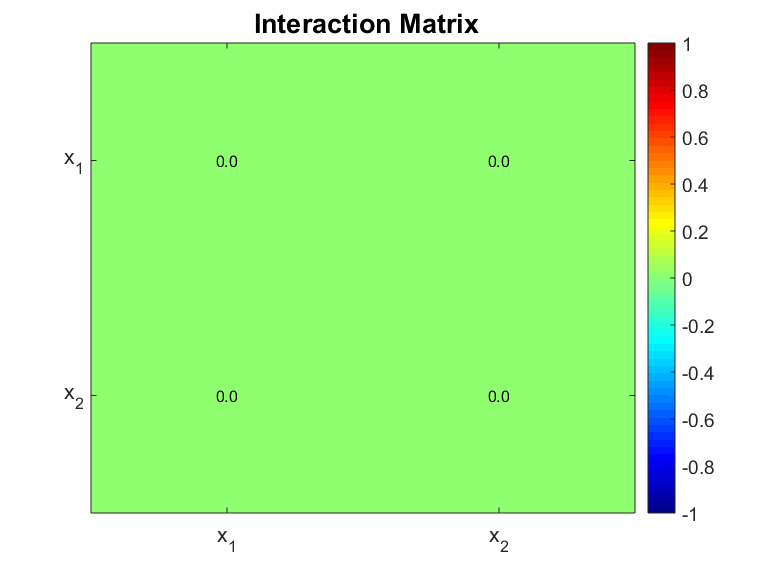
\includegraphics[width = \textwidth]{Stability/Interactions_case_study_1_no_interactions}
		\caption{Interaction matrix of model \eqref{system} with no interactions.}
		\label{case1_no_interactions}
	\end{subfigure}
	~
	\begin{subfigure}[b]{0.45\textwidth}
		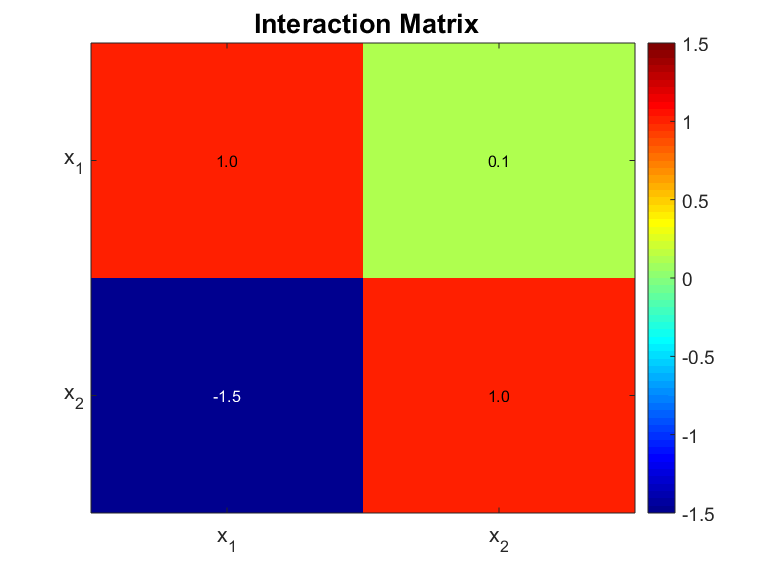
\includegraphics[width = \textwidth]{Stability/Interactions_case_study_1}
		\caption{A non-zero interaction matrix of model \eqref{system}.}
		\label{case1_interactions}
	\end{subfigure}
	\caption{Interaction matrices. Note how the presence of $x_1$ affects very negatively $x_2$ in Figure \ref{case1_interactions}, with respect to other interactions. The terms in the diagonal entries of the matrix represent intraspecies interactions, while the terms off the diagonal represent the interspecies interactions.}
\end{figure} 

\begin{figure}[h]
	\centering
	\begin{subfigure}[b]{0.45\textwidth}
		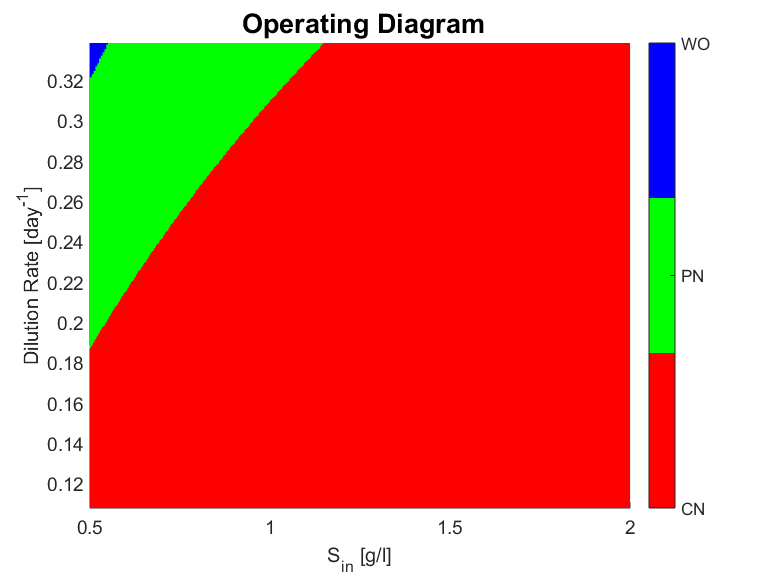
\includegraphics[width = \textwidth]{Stability/OD_case_study_1_no_interactions}
		\caption{Operating diagram of model \eqref{system} with no interactions (interaction matrix represented by figure \ref{case1_no_interactions}).}
		\label{OD_no_interactions}
	\end{subfigure}
~
	\begin{subfigure}[b]{0.45\textwidth}
	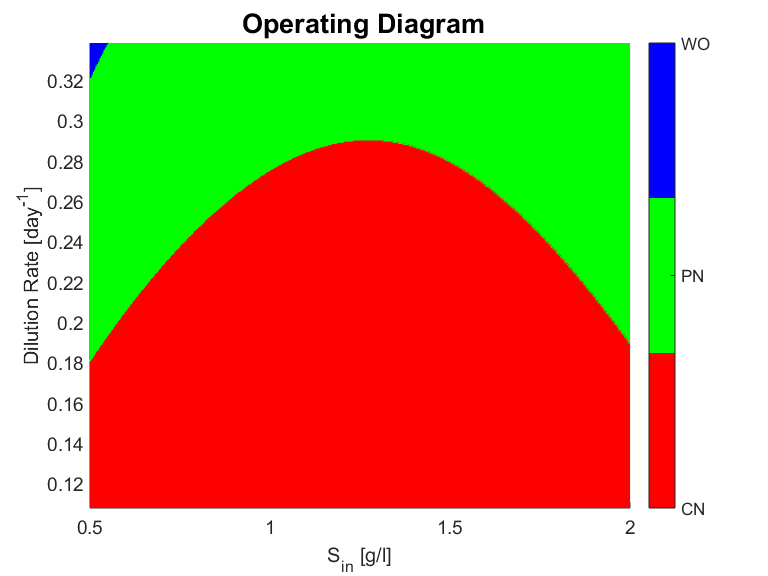
\includegraphics[width = \textwidth]{Stability/OD_case_study_1}
	\caption{Operating diagram of model \eqref{system} with interactions represented by figure \ref{case1_interactions}.}
	\label{OD_interactions}
	\end{subfigure}
	\caption{Note how \ref{OD_interactions} has a much larger zone where partial nitrification takes place. This is due to the negative interaction of $x_1$ on $x_2$.}
	\label{OD_case_1}
\end{figure} 
\clearpage

\textbf{Case study 2: 2 AOB and 2 NOB}

 The case study 2 is based on Dumont \textit{et al.}\cite{Dumont2016} model parameters. They proposed a distribution of parameters obtained from a Bayesian estimation method. Their fit describes well the dynamics of the two most abundant OTU in each functional group, but it still fails to capture the measured substrates dynamics. Kinetic parameters of case study 2 can be seen in Table \ref{kinetic_parameters}. The estimated interaction matrix is shown in Figure \ref{Interaction_1}. A second matrix is presented, which is obtained by the sign change of coefficient $a_{11}$ (Figure \ref{Interaction_2}), and finally a third one is obtained by using a positive value for $a_{12}$ (Figure \ref{Interaction_3}). The idea is to show that qualitatively different outcomes can be obtained by changing one interaction at a time.
 
 \begin{table}[ht]
 	\centering
 	\begin{tabular}{|l|l|l|l|}
 		\hline \rule{0pt}{3.5ex}
 		Case study 2 kinetic parameters & $\mu_i\,[1/day]$ & $K_i\,[mg/L]$ & $\frac{1}{y_i} \, [gr/gr]$ \\ \hline 
 		$x_1 \in G_1$ & 0.828  & 0.147 & 3.85  \\ \hline
 		$x_2\in G_1$ &0.828   & 0.147 &  3.85\\ \hline
 		$x_3\in G_2$ & 0.18 & 0.026 &  100 \\ \hline
 		$x_4\in G_2$ & 0.18 & 0.026 &  100 \\ \hline
 	\end{tabular}
 	\caption{Kinetic parameters of model \eqref{system} from Dumont \textit{et al.} \cite{Dumont2016}}
 	\label{kinetic_parameters}
 \end{table}

\begin{figure}[h]
\begin{subfigure}[b]{0.32\textwidth}
	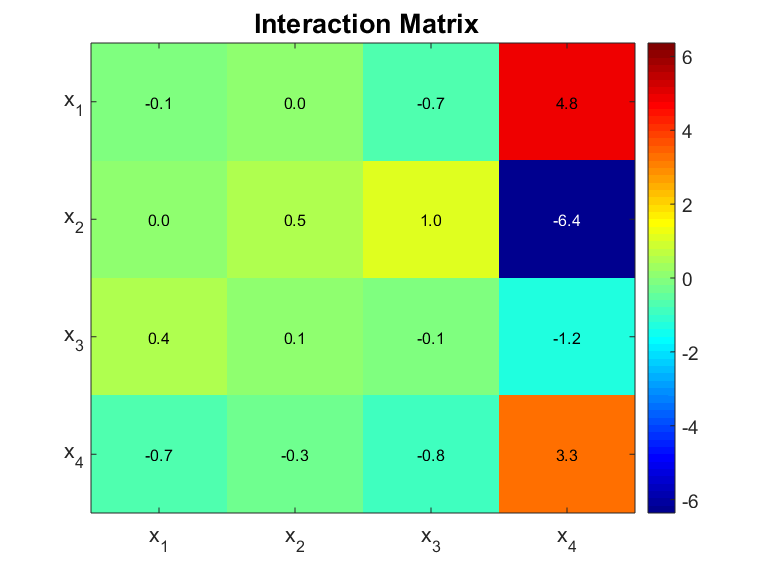
\includegraphics[width=\textwidth]{Stability/Interactions_parameters_Dumont}
	\caption{Originally calibrated interaction matrix.}
	\label{Interaction_1}
\end{subfigure}
~
\begin{subfigure}[b]{0.32\textwidth}
	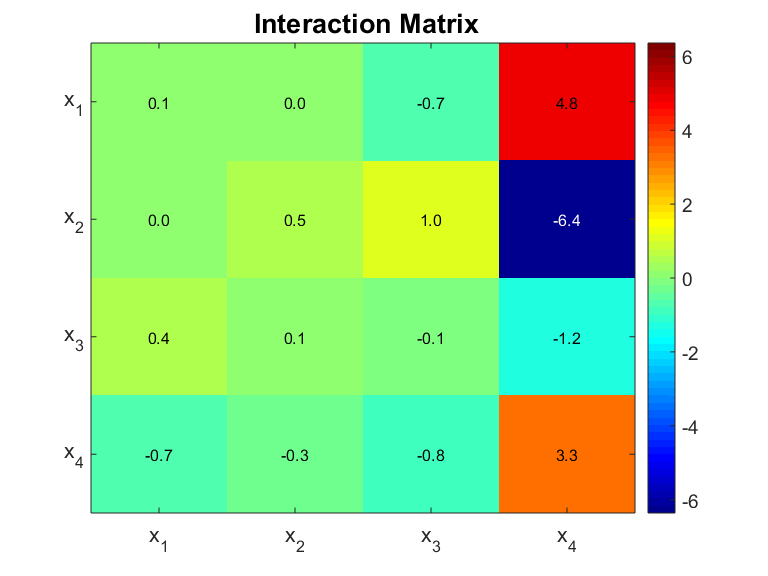
\includegraphics[width=\textwidth]{Stability/Interactions_parameters_modified}
	\caption{Modified interaction matrix with positive intraspecies interaction $a_{11}>0$.}
	\label{Interaction_2}
\end{subfigure}
~
\begin{subfigure}[b]{0.32\textwidth}
	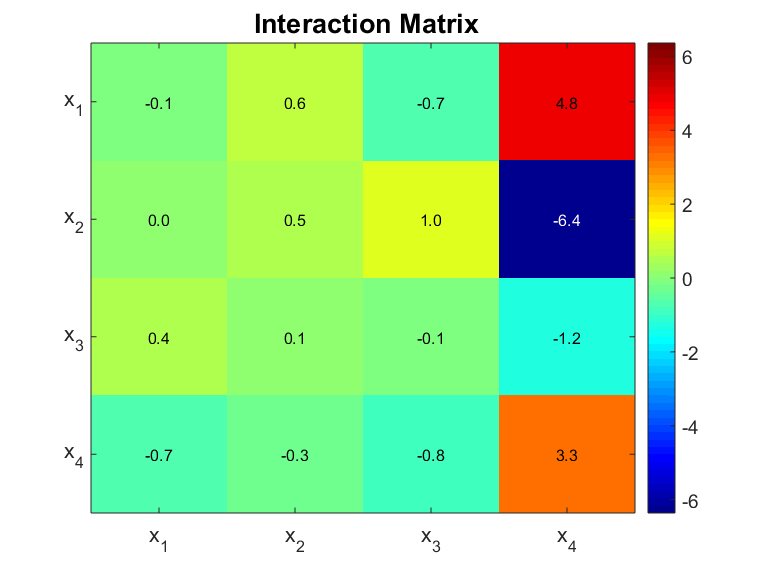
\includegraphics[width=\textwidth]{Stability/Interactions_parameters_modified_2}
	\caption{Modified interaction matrix with positive interspecies interaction  $a_{12}>0$.}
	\label{Interaction_3}
\end{subfigure}
	\caption{Interaction matrices for each case for a consortia of 4 bacterial species where $x_1$ and $x_2$ are AOB and $x_3$ and $x_4$ are NOB. Parameters $a_{11}$ and $a_{12}$ were modified in figures \eqref{Interaction_2} and \eqref{Interaction_3}, respectively.}
	\label{Interactions}
\end{figure} 


\begin{figure}[h]
	\centering
	\begin{subfigure}[t]{0.32\textwidth}
	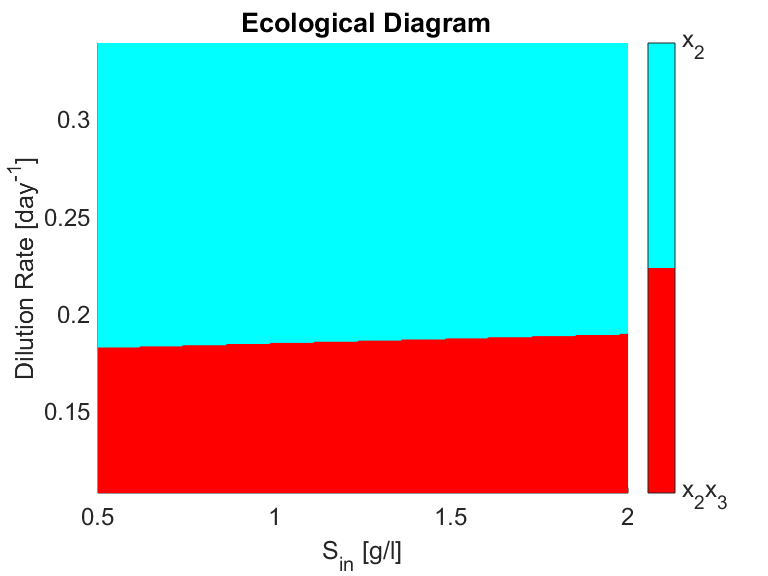
\includegraphics[width=\textwidth]{Stability/ED_parameters_Dumont}
	\caption{Original parameters ecological diagram.}
	\label{ED 1}
	\end{subfigure}
~
	\begin{subfigure}[t]{0.32\textwidth}
	\includegraphics[width=\textwidth]{Stability/ED_parameters_modified}
	\caption{ED from interaction matrix on Figure \ref{Interaction_2}. In the legend 1) and 2) represent the two different stable equilibria in each zone.}
	\label{ED 2}
	\end{subfigure}
~
\begin{subfigure}[t]{0.32\textwidth}
	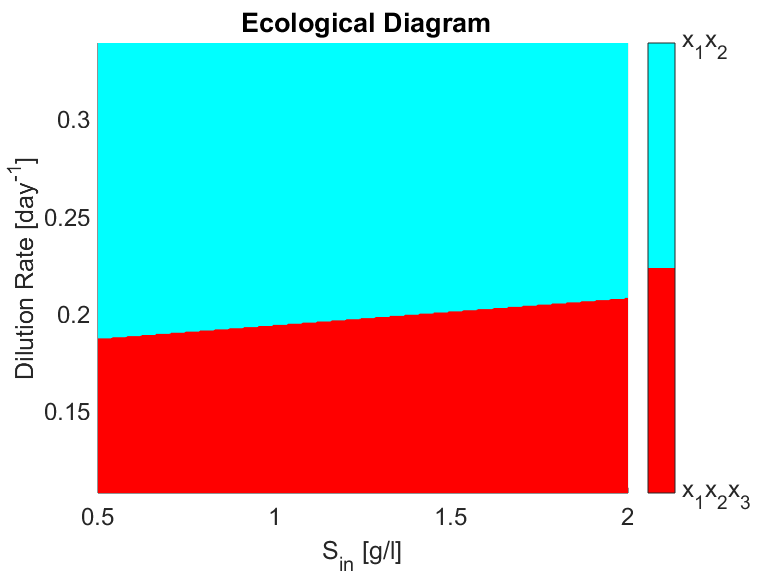
\includegraphics[width=\textwidth]{Stability/ED_parameters_modified_2}
	\caption{ED from interaction matrix on Figure \ref{Interaction_3}.}
	\label{ED 3}
\end{subfigure}

	\caption{Ecological diagrams. The different zones represent the combination of surviving species in the steady state. PN takes place when neither $x_3$ nor $x_4$ are present. CN takes place if $x_3$ or $x_4$ are present. Note that in figure \ref{ED 2} two stable equilibria exist for each zone. }
	\label{ecological_diagrams}
\end{figure}

The ecological diagrams are presented in Figure \ref{ecological_diagrams}, where the legend indicates the species surviving in the zone of the respective colour. In Figure \ref{ED 2}, the system exhibits bi-stability (it is represented in numbering as 1) and 2) of the different possible equilibriums). Note how every zone in figure \ref{ED 2} has two stable equilibria, meaning that the outcome of the system is determined by its initial conditions, particularly interesting is the green zone where either $x_1,x_3$ coexist or only $x_2$ remains, because in operational terms this means that either PN or CN may take place. When compared to Figure \ref{ED 1}, one can see that this change in the interactions of the microbial community can dramatically change the outcome of the reactor in a large operating zone. 

One can see that coexistence in the same functional group is never attained in Figure \ref{ED 1} and \ref{ED 2}, whereas in figure \ref{ED 3} $x_1$ and $x_2$, both AOB, coexist in either partial or complete nitrification. That means that the competitive exclusion principle \cite{lobry2017chemostat} (CEP) does not hold. The CEP roughly states that if two species are growing on the same limiting resource, and their growth laws only depend non decreasingly on the resource, then only one of them will survive in the long run. This is interesting in light of reports on wastewater treatment plants where coexistence between species in nitrifying reactors has been shown \cite{Wagner2002}, thus implying that a more complex growth law (as shown in here) or model structure involving other biological processes is required to include microbial diversity in mathematical models. 

\section*{Remarks}

Model \eqref{system} serves to illustrate that by considering a more complex growth rate that tries to model ecological interactions one might explain differences in reactors operating under similar conditions. It also shows a new mechanism by which the CEP no longer holds and which explains how multiple stable equilibria may appear. Since the gLV model discussed fails to completely capture the dynamics observed in the chemostat experiments \cite{Dumont2016}, the next section proposes a new approach to study interactions.


\section{Generalized approach for modelling interactions}
In the previous sections interactions were modelled as an affine function of the OTU concentration that multiplies a substrate dependent growth equation. More generally the interaction function represents how the growth rate of species $i$ is affected by the concentration of other species, $x$: 

Given a vector $(v_1,\dots,v_n)^\top$ the interaction function $\I$ is denoted as:
\begin{align}
\begin{array}{rc}
\I: \R_+^n \rightarrow & \R_+^n\\
& \\
v \rightarrow & \begin{pmatrix}
I_1(v) \\
I_2(v) \\ 
\vdots  \\
I_n(v)
\end{pmatrix}
\end{array}
\end{align}

Let $f_i(s)$ be a bounded, positive, and continuous function of $s$ (e.g. Monod, Haldane). The growth equation of OTU $i$ becomes:
\begin{align}
	\mu_i(s,x) = f_i(s)I_i(x)
\end{align}
Note $f(s) := (f_1(s),\dots,f_n(s))^\top$.
	\label{growthForm}

Since the growth of a single strain in batch experiments is driven by the substrate concentration, when no interactions are present one should recover expression $f_i(s)$. Therefore if there are no interactions then $I_i(x) = 1$. From this hypothesis, note that $ \lim \limits_{x \rightarrow 0} I_i(x) = 1$ since if there is minimal presence of OTU, interactions can not exist. Furthermore for this study it is assumed that $I_i(\cdot)$ is a continuously differentiable function on $x$. For making explicit all of the former:

\begin{hypo}
	The interaction function $\I$ previously defined satisfies:
	\begin{enumerate}
		\item $	\I \left( (0,\dots,0)^\top \right) = (1,\dots,1)^\top $
		\item There is an open set $\Omega \subset \R^n $ such that $\I \in C^1(\Omega)$.
	\end{enumerate} 
\end{hypo}


Note $J_I(x)$ the Jacobian matrix of function $\mathcal{I}$, then a first order approximation of $\I(\cdot)$ centred at $\bar{x}$ gives: $\I(x) = \I(\bar{x}) + J_I(\bar{x})(x-\bar{x}) + o(\Vert x- \bar{x} \Vert)$. When $\bar{x}= 0$ one recovers the growth expression from the previous section (equations \eqref{gLV growth1} and \eqref{gLV growth2}) implying that $J_I(\bar{0})$ can be seen as the interaction matrix from model \eqref{system}.

\subsection{Unravelling the Interaction Function}

Suppose that the functions $f_i(s)$, and the yields $y_i$ are well-known. By using experimental measurements of $x$, represented by $z(t)$, the objective is to reconstruct function $I(x)$. For doing so, the terms $I_i(x)$ are replaced by controls $u_i(t)$, thus $I_i(x(t)) = u_i(t)$. A control law is obtained by solving a nonlinear optimal tracking problem.	

Consider the observable system \eqref{Controlsystem}, with $y(t) = x(t)$ being the output, because we are observing measurements coming from genetic sequencing.

\begin{align} 
\label{Controlsystem}
\begin{array}{cl}
\dot{x_i} =& \left(f_i(s)u_i(t) -D \right)x_i \quad \forall i \in G_1\\
\dot{x_i} =& \left(f_i(s)u_i(t) -D \right)x_i \quad \forall i \in G_2\\
\dot{s_1} =& \displaystyle (s_{in}-s_1)D + \sum\limits_{i \in G_1}y_{s_1/x_i}f_i(s)u_i(t) x_i  \\
\dot{s_2} = & \displaystyle -s_2D+\sum\limits_{i \in G_1 \cup G_2}y_{s_2/x_i}f_i(s)u_i(t)x_i  \\
\dot{s_3} =&  \displaystyle -s_3D+\sum\limits_{i \in G_2}y_{s_3/x_i}f_i(s)u_i(t) x_i \\
y  =& x
\end{array}
\end{align}	

 Consider the weighted norms defined by positive definite matrices $Q$ and $R$, represented by $\Vert \cdot \Vert_Q$ and $\Vert \cdot \Vert_R$, respectively, and $\bar{u}>0$. The optimal tracking problem is defined as: 

\begin{align}
\label{Optimal Control} \begin{array}{cc} \min &  \int \limits_{0}^{T} \Vert y - z \Vert_Q + \Vert(u -\vec{1}) \Vert_R dt\\
s.t.& 
(x,s_1,s_2,s_3)\mbox{ solution of \eqref{Controlsystem}} \\
&u_i(t) \in [0,\bar{u}]
\end{array}	
\end{align} 

The control $u(t)$ is intended to drive the system to be near a desired output $z(t)$, which in this context are the measurements of the concentrations of OTU. The term $\Vert(u -\vec{1}) \Vert_R$, was added for two reasons:
\begin{itemize}
\item First because the interest is testing the idea that interactions could be driving the system. Therefore adding a penalization in the objective function for each control to remain near $1$ can be seen as an attempt to explain data without any interaction. In other words, if the control terms are found to drift from 1, it means that interactions are necessary to explain the system dynamics.

\item Second, to force a regularized control. Otherwise note that $u$ is linear in \eqref{Controlsystem}, therefore if the integral cost does not have a non-linear expression of $u$ the optimal control will be of a bang-bang type with possibly singular arcs \cite{harmand2019optimal}. Since the objective is to find a differentiable expression of $I(x)$ the addition of the regularization term is deemed necessary.
\end{itemize} 
The problem of approximating the solution of the system to a desired reference ($z$ in this case) is called the optimal tracking problem. For solving such a problem the approach developed by Cimen \textit{et al.} \cite{Cimen2004, Cimen2008} was adapted to our problem. The method proposed involves the resolution of Approximating Sequences of Ricatti Equations (ASRE). It consists of iteratively calculating trajectories of System \eqref{Controlsystem} with a certain control law to later feed a non-autonomous Ricatti differential equation with the resulting trajectory. Then, a new control law that uses the solution of the Ricatti equation is proposed and a new trajectory is calculated. The iteration is stopped when a convergence in the output or  the control is observed.

The control term should remain positive for the system to be well posed (no negative states), and an upper bound was added to represent the fact that life cannot grow infinitely fast. The tracking problem does not consider a constrained control. Nevertheless, the methods of Cimen \textit{et al.}\cite{Cimen2004} were directly used with an explicit constraint in the synthesis of the control. Even though this is probably suboptimal when the control reaches its bounds, one at least is certain about its optimality when the control never reaches its constraints.

Another departure from their method is that in their formulation an approximation of the dynamics for calculating the trajectories is used. They proved that such a linearisation converges to the original dynamics. In the case here presented the linearisation of the dynamics was not necessary.

The change of variable $u_i(t) = v_i(t) + 1$ is used for technical reasons explained in the supplementary material section. This in turn implies $v_i(t) \in [-1,\bar{u}-1]$. The feedback control $v(t)$, will be of the form $v(t) = -R^{-1}\tilde{B}^ \top(t)\left(\tilde{P}(t)x(t)-s_f(t)\right)$. Where matrix $P(t)$ and vector $s_f(t)$ solve differential equations. In the supplementary material it is proved that, thanks to the structure of the system, one only needs to calculate $2n$ differential equations for the synthesis of the control, instead of $(n+3)^2 + (n+3)$ that would imply the direct application of the method, which renders the method- at least theoretically- scalable for a growing number of OTU.

\subsection{Proof of concept}

The approach was tested with data generated by simulating model \eqref{system} using the parameters of the case study 1 (Table \ref{kinetic_parameters_case_study_1}) with interaction matrix given by \eqref{case1_interactions}. In the operating diagram of the same case (figure \eqref{OD_interactions}) the red zone implies complete nitrification, while the green zone means partial nitrification. For integrating the former phenomena in the simulation, the system was simulated for 300 days, and perturbed at day 150 from the CN zone ($(s_{in},D) = (1.25,0.22)$) to a PN zone ($(s_{in},D) = (1.95,0.22)$). Simulations can be seen in figure \ref{synthetic_data}. Note how from day 150 the NOB population (OTU 2) represented in figure \eqref{PC_synthetic_NOB} decreases, which in turn implies a decrease in $s_3$, as seen in figure \eqref{PC_synthetic_metabolites}. In the case where no interactions take place, the OD seen in Figure \ref{OD_no_interactions} implies that $s_3$ would have accumulated all along the trajectory, since the perturbation still remains in the CN zone.


\begin{figure}[h]
	\centering
	\begin{subfigure}{0.32 \linewidth}
 	\includegraphics[width=\linewidth]{proof_of_concept/200525_POC_AOB_plot}
	\caption{AOB.}
	\label{PC_synthetic_AOB}
	\end{subfigure}
	\begin{subfigure}{0.32 \linewidth}
	\centering
	\includegraphics[width=\linewidth]{proof_of_concept/200525_POC_NOB_plot}
	\caption{NOB.}
	\label{PC_synthetic_NOB}
	\end{subfigure}
	\begin{subfigure}{0.32 \linewidth}
	\centering
	\includegraphics[width=\linewidth]{proof_of_concept/200525_POC_metabolites}
	\caption{Metabolites.}
	\label{PC_synthetic_metabolites}
	\end{subfigure}
	\caption{Synthetic data generated by model \eqref{system}, with parameters from case study 1. Note the effects of the increased input $s_{in}$ generated in day 150.}
	\label{synthetic_data}
\end{figure}





%For applying the optimal tracking approach, the choice of matrices $Q$ and $R$ are always of discussion in a quadratic regulator. $Q$ represents the covariance matrix of measurements, while $R$ is subject to interpretations depending on the context: in the case here presented it does not have \textit{a priori} definite meaning. For gaining some insight, its behaviour is studied when $\rho(R) \rightarrow 0$, with $\rho(R)$ being the spectral radius of matrix $R$. In the simulations here presented $Q = I_n$ and $R = \lambda I_n$. In the supplementary material section. $\lambda$ is varied from $10^{-1}$ to $10^{-7}$. The case $\lambda = 10^{-4}$ is shown in here for discussion. 

 For the tracking procedure the functions $f_i(s)$ and the yields $y_i$ were the same as those used for simulating the synthetic data (parameters in table \ref{kinetic_parameters_case_study_1}) and the control is meant to account for the interaction term. The $Q$ and $R$ matrices were $\begin{bmatrix}
 \lambda_1 I_{n_1} &0  \\ 0& \lambda_2 I_{n_2}
 \end{bmatrix}$ and $I_n$, respectively, with $\lambda_1 = 10^{-4}$ and $\lambda_2 = 10^{-5}$ in order to better track the NOB trajectories, since they are less abundant. The results of the procedure to identify interactions can be seen in figure in figure \ref{POC_tracking}. Figures \ref{PC_total_biomass}, \ref{PC_AOB}, and \ref{PC_NOB} show the total biomass concentration, and the trajectories for the OTU belonging to $G_1$ and $G_2$, respectively. It can be seen that the method approaches well the trajectories of the OTU, with a better result for the AOB community, which can be explained by the one order of magnitude difference in their concentrations (which in turn is a consequence of the one order of magnitude difference in their yields). The metabolites concentration represented in figure \ref{PC_metabolites} are in accordance with the simulated: The method is able to reconstruct the metabolites trajectories from the community measurements. 


\begin{figure}[h]
	\centering
	\begin{subfigure}{0.45 \linewidth}
	\includegraphics[width= \textwidth]{proof_of_concept/200525_POC_iter_5_Biomass}
	\caption{Total biomass.}
	\label{PC_total_biomass}
	\end{subfigure}
~
	\begin{subfigure}{0.45 \linewidth}
		\includegraphics[width=\textwidth]{proof_of_concept/200525_POC_iter_5_metabolites}
		\caption{Metabolites. }
		\label{PC_metabolites}
	\end{subfigure}

	\begin{subfigure}{0.45 \linewidth}
		\includegraphics[width=\textwidth]{proof_of_concept/200525_POC_iter_5_AOB_plot_1}
		\caption{AOB biomass.}
		\label{PC_AOB}
	\end{subfigure}
	~
	\begin{subfigure}{0.45 \linewidth}
		\includegraphics[width=\textwidth]{proof_of_concept/200525_POC_iter_5_NOB_plot_1}
		\caption{NOB biomass. }
		\label{PC_NOB}
	\end{subfigure}
\caption{Asterisks represent the synthetic data, while the continuous lines represent the method's output. The method is able to reconstruct the metabolites pattern, from the biomasses concentrations.}
\label{POC_tracking}
\end{figure}



Figure \ref{POC_control} shows the controls and the corrected growth rate for each functional group. The control for each funcional group can be seen in figures \ref{Control AOB no noise} and \eqref{Control NOB no noise}. Note that from the structure of a quadratic regulator, since there is no cost in the final state, the end value is always 1. Figures \ref{AOB_growth_POC} and \ref{NOB_growth_POC} show the resulting growth rates for $AOB$ and $NOB$, respectively, without the control $u_i(t)$. Figures \ref{AOB_growth_control_POC} and \ref{NOB_growth_control_POC} are the complete expression that determines growth rate, that is  $f_i(s(t))u_i(t)x_i(t)$. Note how little the shape changes with respect to figures \ref{AOB_growth_POC} and \ref{NOB_growth_POC}, which might mislead the reader to conclude that the control had reduced effects in the dynamics. The way out of this conundrum is to remember that the control's effects are already included in $x_i(t)$ and $s_i(t)$, and thus in expression $f_i(s(t))x_i(t)$. 

\begin{figure}[h]
	\centering
	\begin{subfigure}{0.45 \linewidth}
		\includegraphics[width=\linewidth]{proof_of_concept/200525_POC_iter_5_Control_AOB_plot_1}
	\caption{Control for the AOB population.}
	\label{Control AOB no noise}
	\end{subfigure}
	\begin{subfigure}{0.45 \linewidth}
		\centering
		\includegraphics[width=\linewidth]{proof_of_concept/200525_POC_iter_5_Control_NOB_plot_1}
	\caption{Control for the NOB population.}
	\label{Control NOB no noise}
	\end{subfigure}

	\begin{subfigure}{0.45 \linewidth}
		\includegraphics[width=\linewidth]{proof_of_concept/200525_POC_iter_5_growth_AOB_plot_1}
		\caption{Growth rate of the model for AOB community.}
		\label{AOB_growth_POC}
	\end{subfigure}
	\begin{subfigure}{0.45 \linewidth}
		\centering
		\includegraphics[width=\linewidth]{proof_of_concept/200525_POC_iter_5_growth_NOB_plot_1}
	\caption{Growth rate of the model for the NOB community.}
	\label{NOB_growth_POC}
	\end{subfigure}

	\begin{subfigure}{0.45 \linewidth}
		\includegraphics[width=\linewidth]{proof_of_concept/200525_POC_iter_5_growth_control_AOB_plot_1}
		\caption{Growth rate of the model for AOB community.}
		\label{AOB_growth_control_POC}
	\end{subfigure}
	\begin{subfigure}{0.45 \linewidth}
		\centering
		\includegraphics[width=\linewidth]{proof_of_concept/200525_POC_iter_5_growth_control_NOB_plot_1}
		\caption{Growth rate of the model for the NOB community.}
		\label{NOB_growth_control_POC}
	\end{subfigure}
	\caption{Control and growth rates resulting from the tracking approach.}
	\label{POC_control}
\end{figure}

%In figure \ref{Comparison_lambda} the different controls obtained by varying $\lambda$ for two species are compared to the interaction function simulated that is $1+A(x(t))$, where $x(t)$ is the synthetic data. One can see that due to this property of the end value becoming 1, the two do not coincide, however, when $\lambda$ is decreased one can see that the control roughly approaches the respective interaction function at the cost of very sharp changes.

%\begin{figure}[h]
%	\centering
%	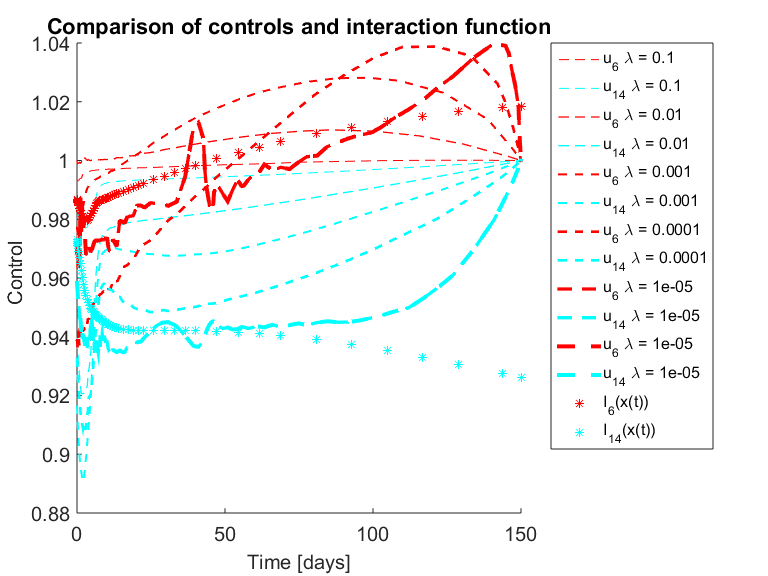
\includegraphics[width=0.5\textwidth]{Synthetic_data//Comparison_different_control}
%	\caption{Obtained controled for different $\lambda$ for two OTU and the interaction function used in the simulation of synthetic data.}
%	\label{Comparison_lambda}
%\end{figure}

\clearpage
\section{Application}
 
%The method was stopped after 10 iterations where each iteration took approximately 800 seconds of computing time in a computer equipped with 8gb of RAM memory and Intel core i3-7100U CPU 2,40 GHz.\iffalse Cette phrase devrait figurer dans la partie précédente ?\fi

The tracking problem was applied to data coming from a nitrification process with experimental conditions described in \cite{dumont2008observers}. For exploring the hypothesis of interactions as drivers of bioreactors performance environmental conditions should be kept as constant as possible. Therefore only data from day $183$ onwards was used because a change in the operating temperature happened at that point, which is known to have an effect on kinetics. For choosing which species belong in which functional group, the procedure described of Ugalde-Salas \textit{et al.} \cite{Ugalde-Salas2019} was used. From day $183$ to day $315$ 31 OTU were identified in the $G_1$ group (AOB) and 5 in the $G_2$ functional group (NOB). 

A first example of the procedure is performed when the classified OTU are regrouped in their assigned functional groups by adding their concentrations. A 5 dimensional dynamical system is obtained, thus there are only two interacting functional biomasses: this case is structurally the same as in the proof of concept, but here a real dataset is used. The same procedure is applied where no regrouping occurs and the system state grows to 39. 

The knowledge of functions $f_i(s)$ was based on a study of nitrification's kinetic parameters\cite{Wiesmann1994}. Particularly given the system's ammonium and nitrite concentration a Monod function (eq \eqref{monod}) was used for $G_1$ and $G_2$ with parameters given in table \ref{kinetic_parameters_application} calculated from the equation of Table 2 of the same article. The yields were fitted to match the nitrogen mass balances. The $Q$ and $R$ matrices were the same as in the proof of concept section, that is $\begin{bmatrix}
\lambda_1 I_{n_1} &0  \\ 0& \lambda_2 I_{n_2}
\end{bmatrix}$ and $I_n$, respectively, with $\lambda_1 = 10^{-4}$ and $\lambda_2 = 10^{-5}$.


\begin{align}
\label{monod} f_i(s) &= \bar{\mu}_2 \dfrac{s_1}{K_1 +s_1} \, \forall i \in G_1 \\
\notag  f_i(s) &= \bar{\mu}_2 \dfrac{s_2}{K_2 +s_2 } \, \forall i \in G_2
\end{align}

\begin{table}[ht]
	\centering
	\begin{tabular}{|l|l|l|l|}
		\hline
		Kinetic Parameters & $\mu_i\,[1/day]$ & $K_i\,[g/L]$ & $\frac{1}{y_i} \, [gr/gr]$ \\ \hline
		$x_1 \in G_1$ & 1.97  & $7\cdot 10^{-1}$ & 4.49  \\ \hline
		$x_2\in G_2$ & 1.87 & $5.4\cdot 10^{-1}$ &  45.51 \\ \hline
	\end{tabular}	
	\caption{A set of kinetic parameters of model \eqref{Controlsystem}.}
	\label{kinetic_parameters_application}
\end{table}
For the reader to gain understanding of the situation, a simulation of the system using the experiments operating parameters ($D$ and $s_{in}$) is presented without control (i.e. $u(t)= 1$) in  figure \ref{u=1 simulation.} nitrite ($s_3$) accumulates all along the trajectory, but when compared to data it is clear that $s_3$ stops accumulating after a while. 

\begin{figure}[h]
	\centering	
	\begin{subfigure}{0.45 \textwidth}
		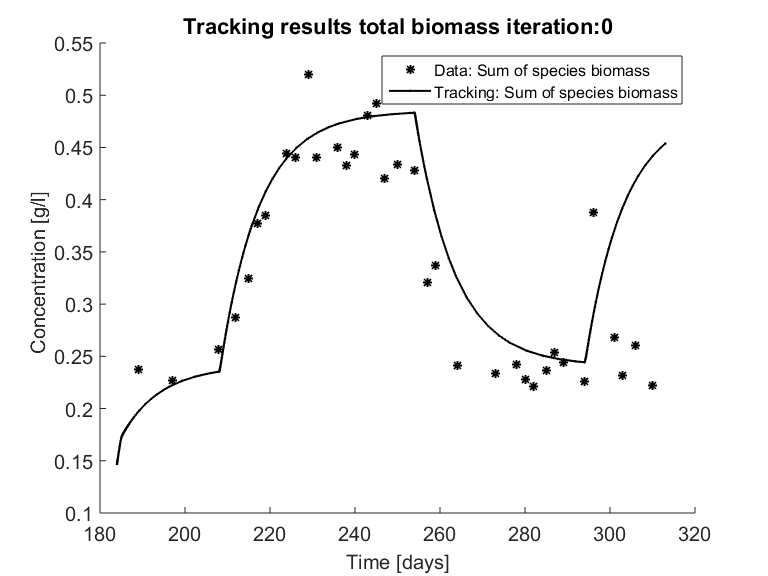
\includegraphics[width=\textwidth]{Application//191218_Reactor_A_Biomass_iter_0}
		\caption{Total Biomass.}
		\label{biomass_no_control}
	\end{subfigure}
	\begin{subfigure}{0.45 \textwidth}
		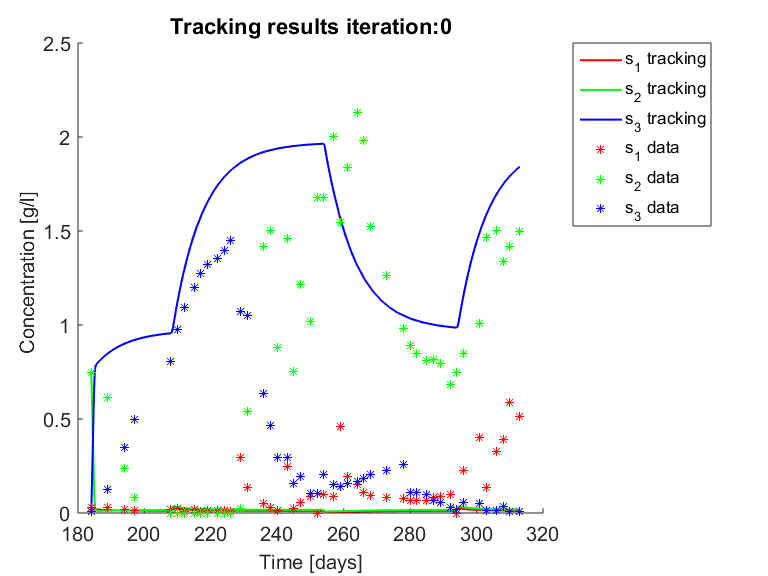
\includegraphics[width= \textwidth]{Application//191218_Reactor_A_metabolites_Iter_0}
		\caption{Metabolites.}
		\label{u=1_metabolites}
	\end{subfigure}
		\caption{Simulation of system \eqref{Controlsystem} when $u=1$, with functions as in \eqref{monod}. Data points are represented by a star. The continuous line represents the simulation.}
		\label{u=1 simulation.}
\end{figure}



\begin{figure}[h]
	\centering
	\begin{subfigure}{0.45 \linewidth}
		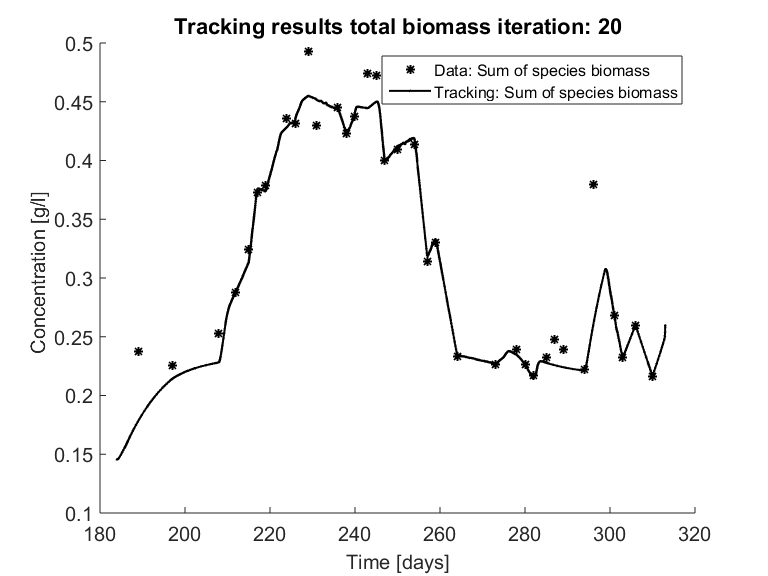
\includegraphics[width= \textwidth]{Application/200407_regroup_OTU_try2_iter_20_Biomass}
		\caption{Total Biomass.}
		\label{Total Biomass application}
	\end{subfigure}
	~
	\begin{subfigure}{0.45 \linewidth}
		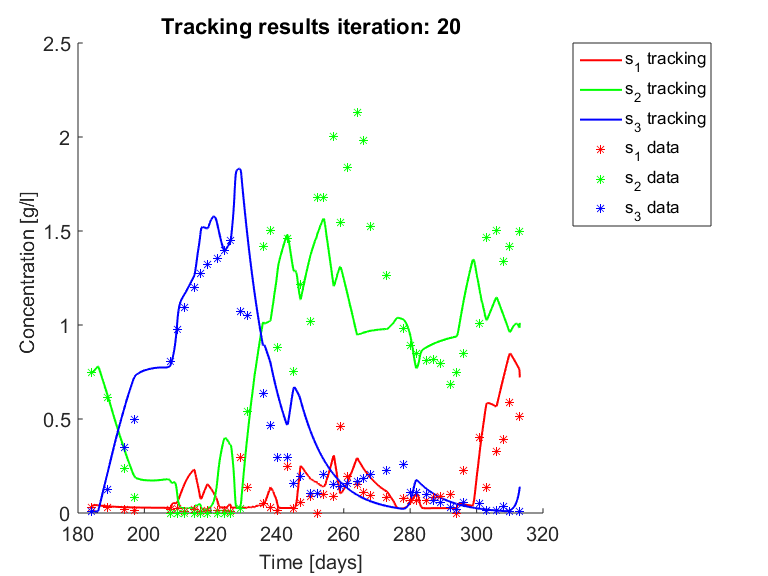
\includegraphics[width=\textwidth]{Application/200407_regroup_OTU_try2_iter_20_metabolites}
		\caption{Metabolites.}
		\label{Metabolites application}
	\end{subfigure}
	\begin{subfigure}{0.45 \linewidth}
		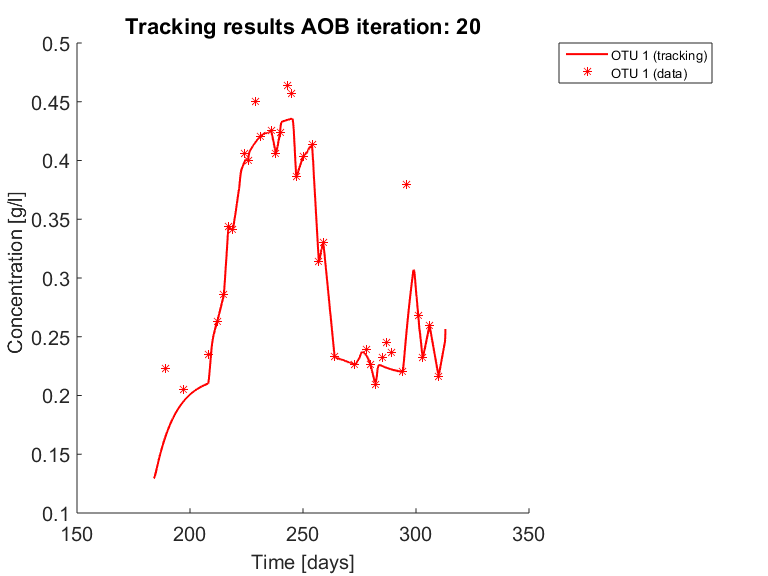
\includegraphics[width=\textwidth]{Application/200407_regroup_OTU_try2_iter_20_AOB_plot_1}
		\caption{AOB biomass.}
		\label{AOB application}
	\end{subfigure}
	~
	\begin{subfigure}{0.45 \linewidth}
		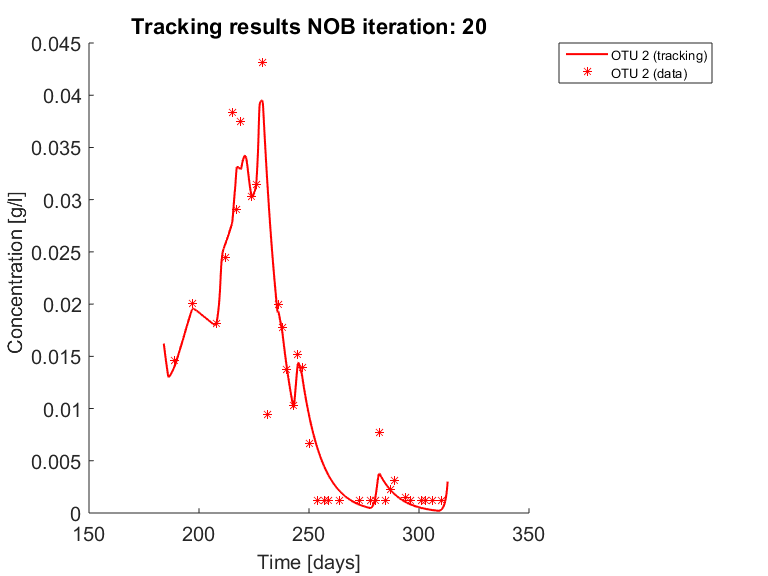
\includegraphics[width=\textwidth]{Application/200407_regroup_OTU_try2_iter_20_NOB_plot_1}
		\caption{NOB biomass.}
		\label{NOB application}
	\end{subfigure}
\caption{Results on applying the tracking method to a nitrification experiment when regrouping OTU in their functional groups. Data points are represented by a star. The continuous line represents the tracking procedure results.}
\label{regroup_results}
\end{figure}


When applying the tracking method one obtains the simulation that can be seen in figure \ref{regroup_results}. The method captures the tendencies of the measured substrates as seen in figure \ref{Metabolites application}. The tracking of each functional group $G_1$ (AOB), and $G_2$ (NOB) can be seen in figures \ref{AOB application} and \ref{NOB application}, respectively. 

The growth rates of each functional group are shown in figure \ref{growth_application}. Note in the case of AOB (figure \ref{AOB_growth_control_application}) the resulting growth rate shows a noisy curve formed by pulses. The behaviour of the NOB community (figure \ref{NOB_growth_control_application}) is qualitatively very similar with somewhat stronger pulses and less noise. The former is to be expected since more OTU were regrouped to compose the AOB biomass, therefore more noise sources were added. 

The same procedure is applied without regrouping. The results on total biomass and metabolites are shown in figures \ref{Total Biomass application all} and \ref{Metabolites application all}, respectively. Both patterns still fit the data, but to a lesser degree of precision when compared to figure \ref{regroup_results}. This can be explained by noting in figure \ref{OTU abudance all} that the most abundant OTU are better tracked, thus the information contained in the least abundant species is not integrated in the model. When looking at the growth rates (figure \ref{growth all}) one again observes pulses for each OTU, note also that most OTU were present only for a fraction of the experiment's duration. 

In both cases, the regrouped and individual tracking, the growth rate varies strongly, raising the question whether the observed pulses are emerging from interactions within the microbial community. When growth rates are compared to the proof of section it seems doubtful that a linear pairwise interaction model such as the gLV model could capture the complexity of the particular chemostat analysed. Perhaps these interactions are not constant through time (as opposed to the gLV model) or a different interaction function should be thought of. However the former questions can not be fully clarified here, because the quality of the genetic sequencing from molecular fingerprints might not be the best when compared to more recent techniques, thus it is unclear if the pulses are due to noise of the measurements.

The interpretation of the correction term as interactions is not the only possible reading. In other contexts the correction term might also be interpreted as a non accounted phenomena ranging from environmental factors (e.g. temperature, pH) to other biological factors (viruses, flock formation, pathogens). Alternative hypothesis for explaining the observed patterns in the microbial community should be considered as well. 

\begin{figure}[h]
	\centering
	\begin{subfigure}{0.45 \linewidth}
		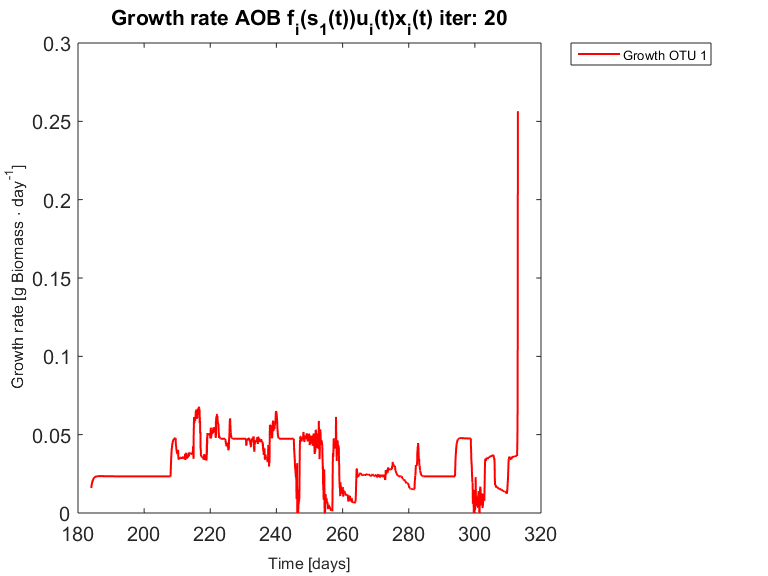
\includegraphics[width=\linewidth]{Application/200407_regroup_OTU_try2_iter_20_growth_control_AOB_plot_1}
		\caption{Growth rate of the model for AOB community.}
		\label{AOB_growth_control_application}
	\end{subfigure}
	\begin{subfigure}{0.45 \linewidth}
		\centering
		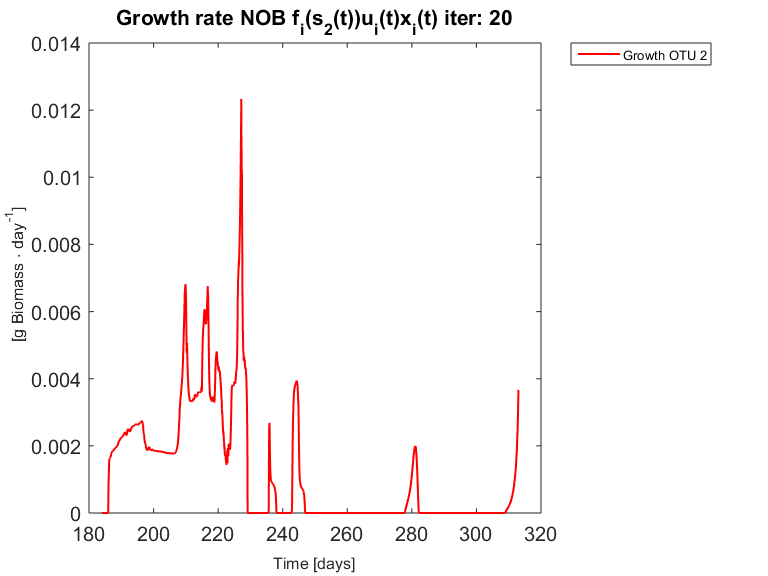
\includegraphics[width=\linewidth]{Application/200407_regroup_OTU_try2_iter_20_growth_control_NOB_plot_1}
		\caption{Growth rate of the model for the NOB community.}
		\label{NOB_growth_control_application}
	\end{subfigure}
	\caption{Obtained growth rates when regrouping OTU in their functional groups.}
	\label{growth_application}
\end{figure}



\begin{figure}[h]
	\centering
	\begin{subfigure}{0.45 \linewidth}
		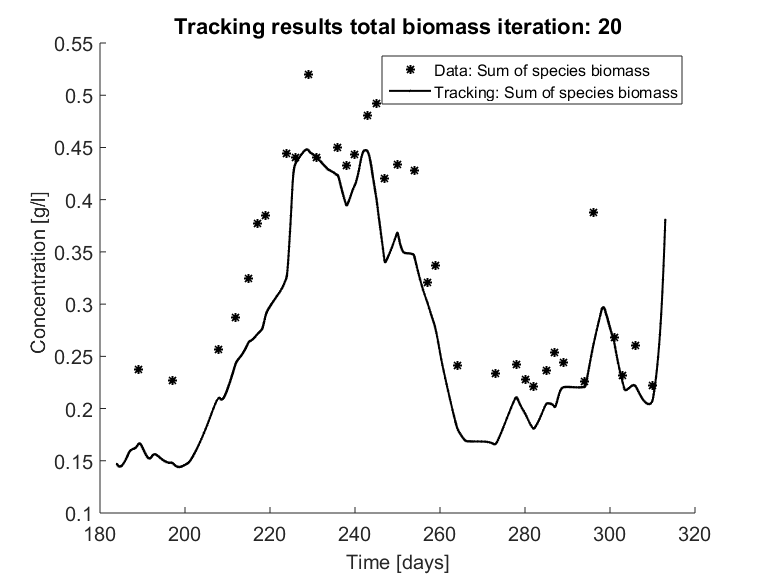
\includegraphics[width= \textwidth]{Application/200407_iter_20_Biomass}
		\caption{Total Biomass.}
		\label{Total Biomass application all}
	\end{subfigure}
	~
	\begin{subfigure}{0.45 \linewidth}
		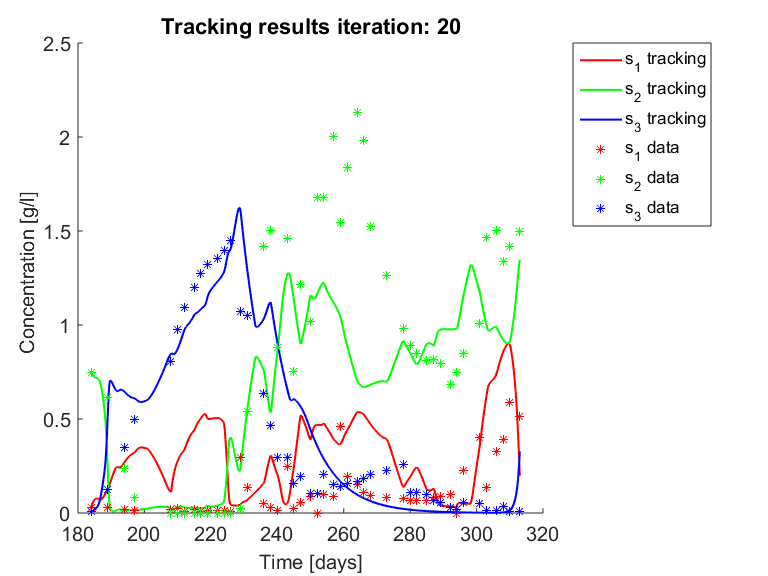
\includegraphics[width=\textwidth]{Application/200407_iter_20_metabolites}
		\caption{Metabolites.}
		\label{Metabolites application all}
	\end{subfigure}
	\caption{Results on applying the tracking method to a nitrification experiment when all OTU are tracked independently. Data points are represented by a star. The continuous line represents the tracking procedure results.}
	\label{all_OTU_results}
\end{figure}

\begin{figure}[h]
	\centering
	\begin{subfigure}{0.45 \textwidth}
		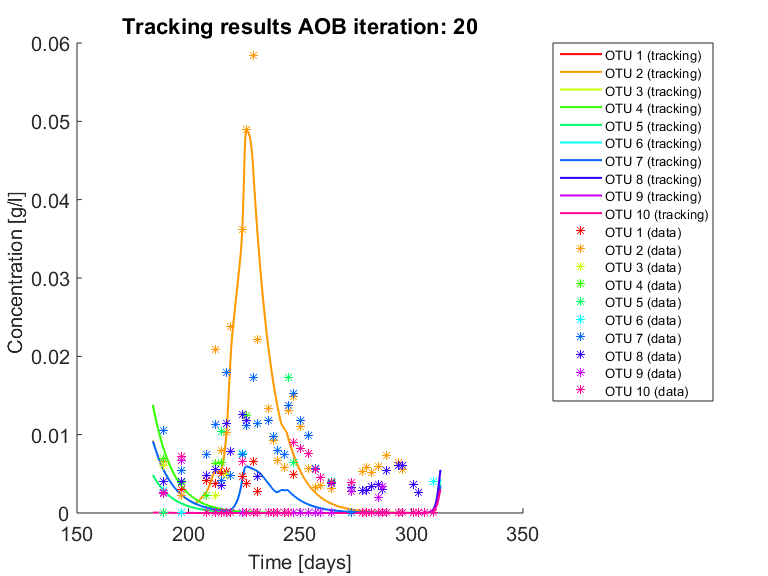
\includegraphics[width =\textwidth]{Application//200407_iter_20_AOB_plot_1}
		\caption{Biomass OTU 1-10 in $G_1$ (AOB) }
	\end{subfigure}
	\begin{subfigure}{0.45 \textwidth}
	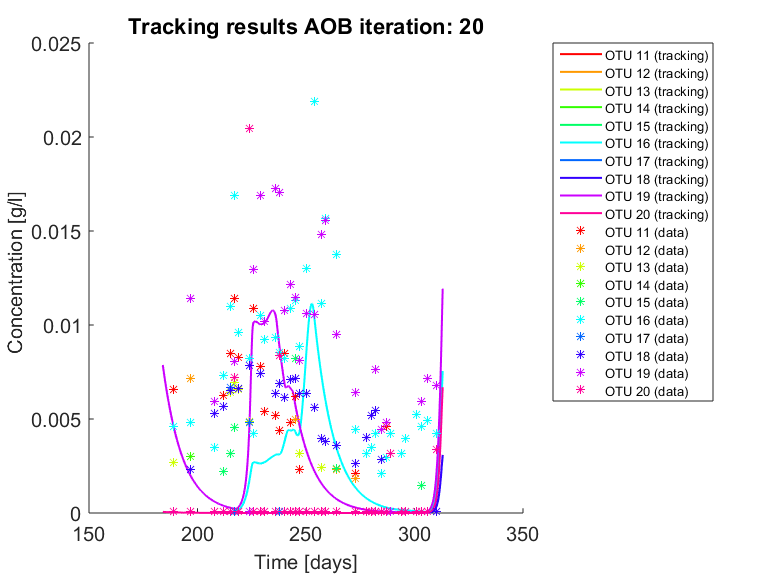
\includegraphics[width =\textwidth]{Application//200407_iter_20_AOB_plot_2}
	\caption{Biomass OTU 11-20 in $G_1$ (AOB) }
	\end{subfigure}
	\begin{subfigure}{0.45 \textwidth}
	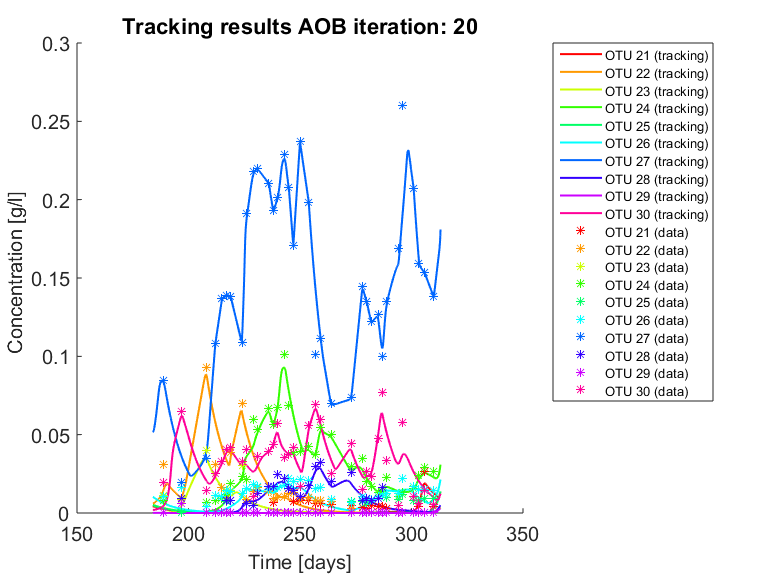
\includegraphics[width =\textwidth]{Application//200407_iter_20_AOB_plot_3}
	\caption{Biomass OTU 21-30 in $G_1$ (AOB) }
	\end{subfigure}
	\begin{subfigure}{0.45 \textwidth}
	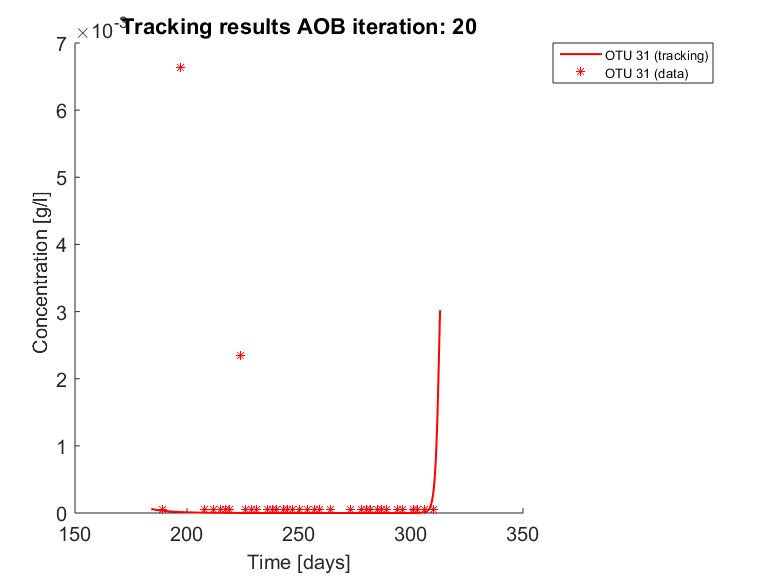
\includegraphics[width =\textwidth]{Application//200407_iter_20_AOB_plot_4}
	\caption{Biomass OTU 31 in $G_1$ (AOB) }
	\end{subfigure}
	\begin{subfigure}{0.45 \textwidth}
	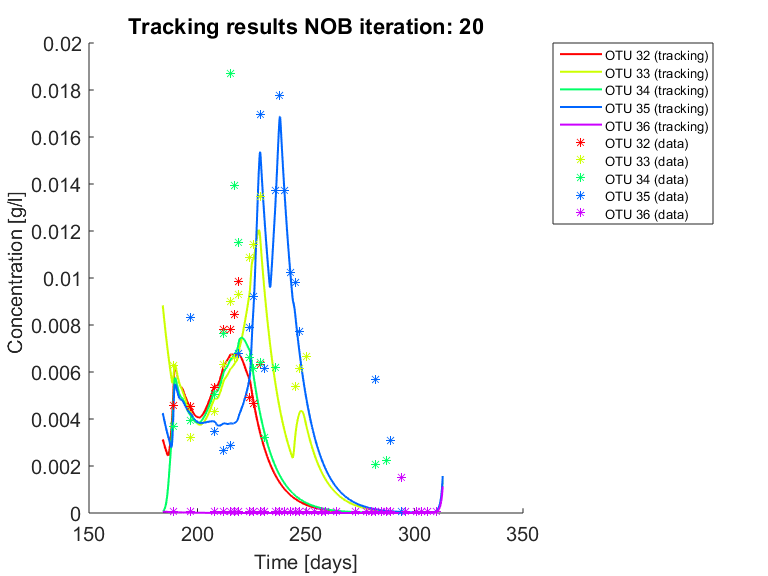
\includegraphics[width =\textwidth]{Application//200407_iter_20_NOB_plot_1}
	\caption{Biomass OTU 32-36 in $G_2$ (NOB) }
	\end{subfigure}
	\caption{Tracking results when all OTU are tracked independently. Note the different y-axis scales of each plot.}
	\label{OTU abudance all}
\end{figure}


\begin{figure}[h]
	\centering
	\begin{subfigure}{0.45 \textwidth}
		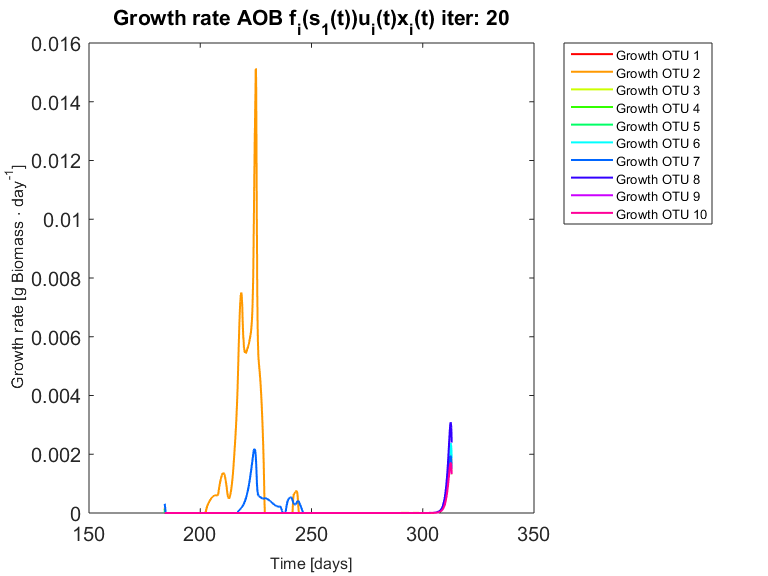
\includegraphics[width =\textwidth]{Application//200407_iter_20_growth_control_AOB_plot_1}
		\caption{Growth rate of OTU 1-10 in $G_1$ (AOB) }
	\end{subfigure}
	\begin{subfigure}{0.45 \textwidth}
		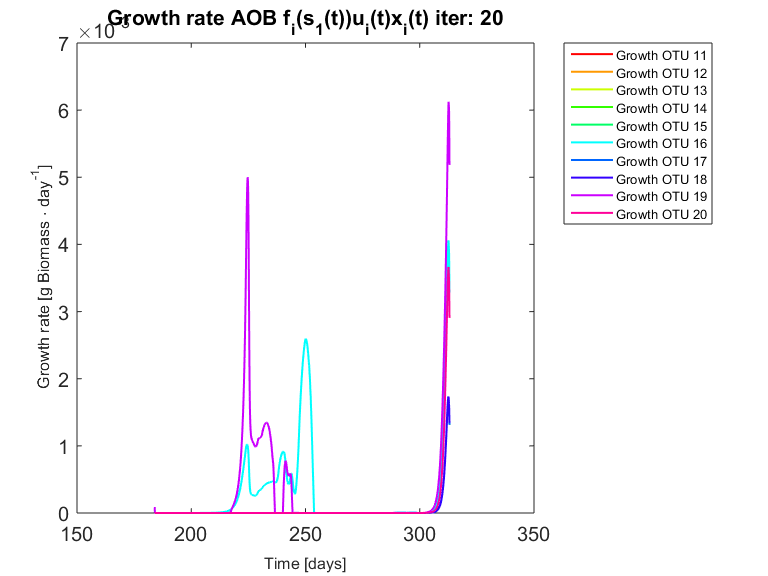
\includegraphics[width =\textwidth]{Application//200407_iter_20_growth_control_AOB_plot_2}
		\caption{Growth rate of OTU 11-20 in $G_1$ (AOB) }
	\end{subfigure}
	\begin{subfigure}{0.45 \textwidth}
		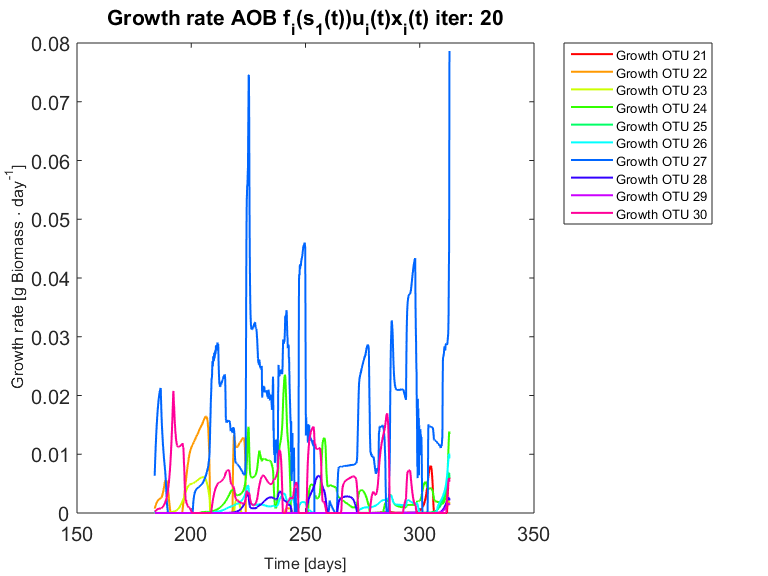
\includegraphics[width =\textwidth]{Application//200407_iter_20_growth_control_AOB_plot_3}
		\caption{Growth rate of OTU 21-30 in $G_1$ (AOB) }
	\end{subfigure}
	\begin{subfigure}{0.45 \textwidth}
		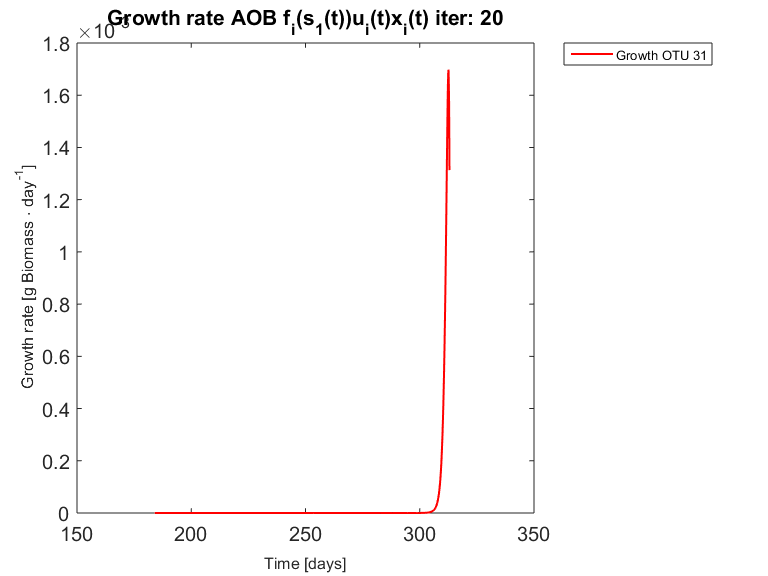
\includegraphics[width =\textwidth]{Application//200407_iter_20_growth_control_AOB_plot_4}
		\caption{Growth rate of OTU 31 in $G_1$ (AOB) }
	\end{subfigure}
	\begin{subfigure}{0.45 \textwidth}
	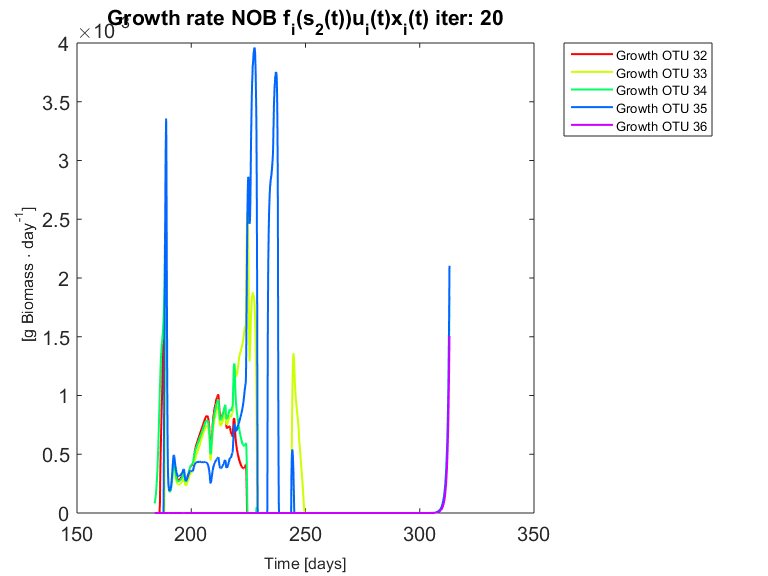
\includegraphics[width =\textwidth]{Application//200407_iter_20_growth_control_NOB_plot_1}
	\caption{Growth rate of OTU 32-36 in $G_2$ (NOB) }
	\end{subfigure}
	\caption{Growth rates obtained for each OTU when applying the tracking procedure without aggregation.}
	\label{growth all}
\end{figure}


\clearpage
\section{Conclusions and Perspectives}

Last decades advances in genetic sequencing and microbial ecology have opened a gap for modellers in biochemical processes to integrate this valuable information. Considering the success of mass balance models to predict and pilot bioreactors, new models should be built upon them. This article exposed what can be gained from combining population-based models as used in ecology with functional group based approaches as used in bioengineering. The analysis of the gLV model proposed by Dumont \textit{et al.} \cite{Dumont2016} already shows that such a combination can give way to models that include bi-stability, coexistence within a functional group, and unintuitive operational insights such as raising the input ammonium $s_{in}$ to achieve partial nitrification. The increased number of parameters of this particular model obviously hinders its potential application, but it surely helps to illustrate what can be gained by joining both types of models. The mathematical analysis focused on the particular case of pairwise interactions, which can be seen as a first order approximation of the introduced concept of interaction function. This opens the question for a broader class of interaction functions that could represent well complex microbial ecosystems, particularly bioreactors. 

In that line of reasoning, in order to understand what this interaction function should look like, a data-driven approach was presented. It can be simply described as correcting the growth rate expression of each individual species in a mass balance model, by explicitly assuming a control loop on the growth rate depending on the species state variables and the measured abundances. The reconstructed growth rates seem to consist of pulses, suggesting that a form of a possible interaction function should reproduce this behaviour, however since the quality of molecular fingerprints is not the best, one can not discard the possibility that this is due to noise of the measurements. In spite of the former, one is able to recover the substrates dynamics, implying that the hypothesis of microbial interactions as drivers of a bioprocess, in the form of feedback loops affecting each others growth rates, is not far-fetched. 

The use of the tracking technique can be applied in a straightforward manner to already existing models in mixed homogeneous bioreactors, under the condition that the the microbial species have already been identified with a particular functionality of the system. Even though the tracking model was proposed for a chemostat setting as a way to correct a substrate limited expression, the method could be used in contexts where less information on the growth function of microbes is known. If one supposes nothing on the growth expression but the fact that is bounded (life cannot grow infinitely fast) the model becomes a linear model and one recovers a classic quadratic regulator for linear systems. Nevertheless, even in the former case, the synthesis of the optimal bounded control remains an open theoretical challenge. One might bypass this issue of the current control scheme by, for example, a very thorough use of the Pontryagin maximum principle for the synthesis of the control. In a more general view the reconstruction of the growth function in chemostat systems is already subject to problems of identifiability\cite{Dochain2003}, integrating genetic sequencing could provide a path for more certainty in model calibration. 


\section{Codes}

All the codes can be recovered from the following repository \url{https://github.com/paus-5/Class-and-Track}.
\section{Acknowledgements}
 The authors would like to thank Alain Rapaport for the exchanges and comments. This work was financed by project Thermomic ANR-16-CE04-0003.

\section{Supplementary Material}

\subsection{Proofs of \cref{l1} and \cref{theoWellPosedness}}

\systembounds* 

\begin{proof}
	Define 
	\begin{align}
	z_1 &: = \sum \limits_{i \in G_1} \frac{1}{y_i}x_i + s_1  \\
	z_2 &: = \sum \limits_{i \in G_2} \frac{1}{y_i}x_i + s_1 + s_2 \\
	z_3 &: = s_1 + s_2 + s_3
	\end{align} 
	
	Computing $\dot{z_{1}}$ one gets:
	\begin{align*}
	\dot{z_{1}} &=\sum \limits_{i \in G_1} \frac{1}{y_i}\dot{x_i} + \dot{s_1} \\
	& = \sum \limits_{i \in G_1} \frac{1}{y_i}\left(\mu_i(s_1,x) -D \right)x_i + (s_{in}-s_1)D-\sum\limits_{i \in G_1}\frac{1}{y_i}\mu_i(s_1,x) x_i   \\
	&= 	D\left(-\sum \limits_{i \in G_1} \frac{1}{y_i}x_i - s_1 + s_{in}\right)  \\
	& = D(s_{in} - z_1)
	\end{align*}
	
	Define $\bar{s} =\max\{s_{in}(t) | t\geq 0\}$ and consider the differential equation:
	
	\begin{align}
	\label{compareEquation}
	\begin{array}{l}
	\dot{w} = D(\bar{s} - w) \\
	w(0) = \sum \limits_{i \in G_1} \frac{1}{y_i}x_i(0) + s_1(0)
	\end{array}
	\end{align}
	
	If there is a time interval $H$ such that $t^*\in H  \Rightarrow D(t^*) = 0$, then $z_1$ is constant and therefore bounded by  the value of the solution in $z(t^*)$. 
	If $D(t) > 0$, then $w = \bar{s}$ is a stable asymptotic equilibrium. Define $M_1 :=  \max\{w(0),\bar{s}\}$. If $ w(0) > \bar{s}$ then by the Picard-Lindeloff theorem $ \forall t \; \dot{w}(t) < 0 $, otherwise it would cross the solution of the initial value problem \eqref{compareEquation} with starting point $\bar{s}$ , therefore $w(t) \geq \bar{s}$. The same reasoning may be applied if $ w(0) < \bar{s}$. One concludes that $ w(t) \leq M_1 $. 
	
	Consider  
	\begin{align}
	\label{z1} \begin{array}{l}
	\dot{z_1} =  D(s_{in} - z_1)\\
	z_1(0) = \sum \limits_{i \in G_1} \frac{1}{y_i}x_i(0) + s_1(0)
	\end{array} 
	\end{align}
	From a comparison lemma (see chapter 3 \cite{Khalil1996}), the solution of \eqref{z1} is bounded by $w$ and therefore $z_1(t) \leq M_1$.
	
	By defining $M_2 = \max\left \{ \displaystyle \sum \limits_{i=n_1 +1 }^{n} \frac{1}{y_i}x_i(0) + s_1(0) +s_2(0), \bar{s} \right\}$, and $M_3 =\max\left \{ s_1(0) +s_2(0) + s_3(0), \bar{s} \right\} $ and noting that $z_2(t)$ and $z_3(t)$ satisfies the same differential equations as $z_1$ the above reasoning may be applied and one has the desired bounds.
\end{proof}


\wellposedness*

\begin{proof}
	If any coordinate of the solution becomes zero, then it's derivative is either zero, or positive. The bound will follow from Lemma \ref{l1}.
	
	Note that for any $i \in \{1,\dots, n\} $ if $x_i = 0$ then $\dot{x_{i}} = 0$, therefore all solutions of system \eqref{system} with initial condition $x_i(t_0) = 0$ remain in these planes. By the Picard Lindeloff theorem a solution starting in $int(\Omega)$ cannot cross these planes, therefore $x_i(t)\geq 0$ for $t \geq 0$.
	
	If $s_1 = 0$, then $\dot{s_1} = Ds_{in} > 0$. Therefore $s_1(t) \geq 0$.
	
	If $s_2 = 0$ then note first that by adding both inequalities from Lemma \eqref{l1}:
	\begin{align*}
	\sum \limits_{i \in G_1 \cup G_2}  \frac{1}{y_i} x_i + 2s_1 + s_2 \leq M_1 + M_2 
	\end{align*}
	let $\bar{k} = \min \left\{ \frac{1}{y_i}  : \; i\in [n] \right \}$ and since $s_1,x_i \geq 0$ one has:
	\begin{align*}
	\Rightarrow \bar{k} \sum  \limits_{i = 1}^{n}   x_i  \leq M_1 + M_2  \\
	\Leftrightarrow \bar{k} \sum  \limits_{i = 1}^{n}   \vert x_i \vert  \leq M_1 + M_2  \\
	\Leftrightarrow \bar{k} \Vert x \Vert_1  \leq M_1 + M_2  \\
	\Rightarrow   \bar{k} \Vert x \Vert_{\infty} \leq M_1 + M_2
	\end{align*}
	
	
	Define $M := \dfrac{\bar{k}}{M_1 + M_2}$, and let $A$ be a matrix such that $\Vert A \Vert_{\infty} \leq M$. Since
	\begin{align*} \Vert Ax \Vert_{\infty} \leq 1 \Rightarrow   (1 + A_{i\bullet}x) \geq 0 \quad \forall i \in [n]
	\end{align*}
	
	and $\Vert Ax \Vert_{\infty} \leq \Vert A \Vert_{\infty} \Vert x\Vert_{\infty} \leq M \frac{1}{M}$. One has proven that:
	\begin{align}
	\label{Bound1}  \;   (1 + A_{i\bullet}x) \geq 0  \quad \forall i \in [n]
	\end{align} 
	
	Therefore $\dot{s_2} = \displaystyle \sum \limits_{i \in G_1 } \frac{1}{y_i}\mu_i(s_1,x)x_i =  \sum \limits_{i \in G_1 } \frac{1}{y_i}\bar{\mu_i}f_i(s)(1+A_{i \bullet }x)x_i \geq 0$. Therefore $s_2(t) \geq 0$.
	
	Note that since one has proven that $s_2 \geq 0$, bound \eqref{Bound1} is valid for any time, and not only when $s_2 = 0$. 
	If $s_3 = 0$ then $\dot{s_3} = \sum \limits_{i \in G_2 }^{n}\frac{1}{y_i}\mu_i(s_2,x)\geq 0$. Therefore $s_3 \geq 0$.
	
	For the boundedness it suffices to notice from \cref{l1} that the sum of positive elements is bounded, therefore each element is bounded.
\end{proof}

\subsection{Deduction of  Equilibrium points}


Recall that 

\begin{align}
f_i(s) = \begin{cases}
\bar{\mu}_i \dfrac{s_1}{K_i + s_1} \quad \forall i \in G_1 \\
\bar{\mu}_i \dfrac{s_2}{K_i + s_2} \quad \forall i \in G_2
\end{cases}
\end{align}

then $\mu(x,s) = \diag(f(s))(1_{n\times 1} + Ax)$ thus, system \eqref{system} is rewritten as follows. 

%\begin{align}
%\label{Eq1}	\dot{x} = & \diag(x)(\diag(f(s))(1_{n\times 1} + Ax) - D_{n\times 1}) \\
%\label{Eq2}	\dot{s_1} = & (s_{in}-s_1)D + \begin{bmatrix}
%-(1_{n_1\times 1} +A_1x) \\0
%\end{bmatrix}^\top \diag(k) \diag(f(s))x \\
%\label{Eq3}	\dot{s_2} = & -s_2D+
%\begin{bmatrix}
%1_{n_1\times 1} +A_1x \\ -(1_{n_2\times 1} +A_2x)
%\end{bmatrix}^\top \diag(k) \diag(f(s))x \\	
%\label{Eq4}	\dot{s_3} = & -s_3D+\begin{bmatrix}
%0	\\(1_{n_2\times 1} +A_2x) 
%\end{bmatrix}^\top \diag(k) \diag(f(s))x 
%\end{align} 
\begin{align}
\tag{\ref{Eq1}}	\dot{x} = & \diag(\mu(x,s) - D_{n\times 1})x \\
\tag{\ref{Eq2}}	\dot{s_1} = & (s_{in}-s_1)D + Y_{1\bullet} \diag(\mu(x,s))x \\
\tag{\ref{Eq3}}	\dot{s_2} = & -s_2D+
Y_{2\bullet} \diag(\mu(x,s))x\\	
\tag{\ref{Eq4}}	\dot{s_3} = & -s_3D+Y_{3\bullet} \diag(\mu(x,s))x 
\end{align} 

Recall $\mathcal{J}$ the set of non-active coordinates. Let $M$ be the matrix defined by taking out the $\mathcal{J}$ columns of the identity matrix of size $n$. When $M$ multiplies from the left it adds rows of zeros to the multiplied matrix in the $\mathcal{J}$ coordinates. When matrix $M$ multiplies from the right it takes out the $\mathcal{J}$ columns of the multiplied matrix. When $M^\top$ multiplies from the left it takes out the $\mathcal{J}$ rows of the multiplied matrix. When $M^{\top}$ multiplies from the right it adds columns of zeros to the multipled matrix in the $\mathcal{J}$ coordinates. This gives the following relationships:
	\begin{align}
	x^{eq} = Mx^{act} \\	
	f^{act}(s) = M^{\top}f(s) \\
	\mu^{act}(x,s) = M^{\top}\mu(x,s)\\
	Y^{act} = YM \\
	M^\top M = I_{n^{act}}
	\end{align}.   

From equation \eqref{Eq1} equilibrium points satisfy: 

\begin{align}
x_i = 0 \vee (\diag(f(s))(1_{n\times 1} + Ax) - D_{n\times 1})_i = 0 \quad \forall i \in [n] \\
\Rightarrow  (\diag (f(s))(1_{n\times 1}+ Ax) - D_{n\times 1})_i = 0 \quad \forall i \in [n]\setminus \mathcal{J} \\
\Leftrightarrow f_i(s)(1 + A_{i\bullet}x) - D = 0 \quad \forall i \in [n]\setminus \mathcal{J} \label{Extinction}
\end{align} 

note that $\forall j \in \mathcal{J}, \; x^{eq}_j = 0 $ therefore the coefficients $a_{ij}$ play no role in equation \eqref{Extinction} and one can rewrite equation \eqref{Extinction} as 
\begin{align} 
\label{mu=D}\mu^{act}(x,s) = \diag(f^{act}(s))(1_{n^{act}\times 1} + A^{act}x^{act}) = D_{n^{act} \times 1} 
\end{align}

From hypothesis \ref{inverse hypothesis} matrix $A^{act}$ has an inverse. This gives the following formula
	\begin{align}
	x^{act} = (A^{act})^{-1}(\diag(f^{act}(s))^{-1}D_{n^{act}\times 1} - 1_{n^{act}\times 1}) \tag{\ref{EqSome}}
	\end{align} 



Note as well that at the equilibrium, $s_3$ can be defined in terms of $s_1$, $s_2$ and $s_{in}$. This is done by adding equations \eqref{Eq2}, \eqref{Eq3},  and \eqref{Eq4} which gives :

\begin{align}
s_{in} = s_1+s_2+s_3 \tag{\ref{s1s2s3}}
\end{align}

\subsubsection{Both functional groups are present}

The case where in each functional group remains at least one OTU is represented by Hypothesis \ref{hypothesis CN}.

By replacing $x^{eq} = Mx^{act}$ in equation \eqref{Eq2} yields


\begin{align}
(s_{in}-s_1)D + Y_{1\bullet} \diag(\mu(x,s))Mx^{act}  = 0 \\
(s_{in}-s_1)D + Y^{act}_{1\bullet} \diag(\mu^{act}(x,s))x^{act}  = 0 
\end{align}

Replacing \eqref{mu=D} gives: 

\begin{align} 
(s_{in}-s_1)D + Y^{act}_{1\bullet} \diag(D_{n^{act}\times 1})x^{act}  = 0  \\
(s_{in}-s_1) + Y^{act}_{1\bullet} x^{act}  = 0  \\
\label{s1Equilibria} (s_{in}-s_1) + Y^{act}_{1\bullet}(A^{act})^{-1}(\diag(f^{act}(s))^{-1}D_{n^{act}\times 1} - 1_{n^{act}\times 1}) = 0
\end{align} 

For notation and indexing purposes it is useful to define: 
\begin{align}
B := Y^{act}_{1\bullet} (A^{act})^{-1}M^\top.
\end{align}
(note $B_j = 0 \, \forall j \in \mathcal{J}$) and equation \eqref{s1Equilibria} reads as follows:

\begin{align}
(s_{in}-s_1) + Y^{act}_{1\bullet}(A^{act})^{-1}\underbrace{M^\top M}_{I_{n^{act}}}(\diag(f^{act}(s))^{-1} D_{n^{act}\times 1} - 1_{n^{act}\times 1}) = 0\\
\displaystyle s_{in} - s_1 + \sum \limits_{i \in G_1} B_i \left(\dfrac{K_i+s_1}{\bar{\mu_i}s_1}D - 1 \right) + \sum \limits_{i \in G_2 } B_i \left(\dfrac{K_i+s_2}{\bar{\mu_i}s_2}D - 1 \right)= 0 \label{to_be_reused}\\
\displaystyle s_{in} - s_1 + \sum \limits_{i \in G_1 } DB_i \dfrac{K_i+s_1}{\bar{\mu_i}s_1}+ \sum \limits_{i \in G_2 } DB_i \dfrac{K_i+s_2}{\bar{\mu_i}s_2} - \sum \limits_{i \in G_1 \cup G_2}B_i= 0 \quad /\cdot s_1s_2 
\\
\displaystyle s_1s_2 s_{in}- s^2_1s_2 + \sum \limits_{i \in G_1} s_2DB_i \dfrac{K_i+s_1}{\bar{\mu_i}}+ \sum \limits_{i \in G_2 } s_1DB_i \dfrac{K_i+s_2}{\bar{\mu_i}} - s_1s_2\sum \limits_{i \in G_1 \cup G_2}B_i= 0 \\
\displaystyle s_1s_2 s_{in}- s^2_1s_2 + s_2\sum \limits_{i \in G_1 } \frac{DB_iK_i}{\bar{\mu_i}}+s_1s_2\sum \limits_{i \in G_1 } \frac{DB_i}{\bar{\mu_i}}+ s_1\sum \limits_{i \in G_2 } \frac{DB_iK_i}{\bar{\mu_i}} + s_1s_2\sum \limits_{i \in G_2 } \dfrac{DB_i}{\bar{\mu_i}} - s_1s_2\sum \limits_{i \in G_1 \cup G_2}B_i= 0 \\
\displaystyle s_2\left(s_1s_{in} - s^2_1 + \sum \limits_{i \in G_1} \frac{DB_iK_i}{\bar{\mu_i}} +s_1\sum \limits_{i \in G_1 } \dfrac{DB_i}{\bar{\mu_i}}+s_1\sum \limits_{i \in G_2 } \dfrac{DB_i}{\bar{\mu_i}}  - s_1\sum \limits_{i \in G_1 \cup G_2}B_i  \right) = - s_1\sum \limits_{i \in G_2 } \frac{DB_iK_i}{\bar{\mu_i}} \\
\displaystyle s_2\left( - s^2_1 +s_1\left(s_{in}+\sum \limits_{i \in G_1 \cup \in G_2 } B_i\left(\dfrac{D}{\bar{\mu_i}}-1\right) \right) + \sum \limits_{i \in G_1} \frac{DB_iK_i}{\bar{\mu_i}}\right) = - s_1\sum \limits_{i \in G_2 } \frac{DB_iK_i}{\bar{\mu_i}}
\end{align}
 
and so we arrive to formula
\begin{align}
s_2 = \frac{s_1}{b_1s_1^2+b_2s_1+b_3} \tag{\ref{S2(S1)}}
\end{align}

where
\begin{align}
\displaystyle b_1 & =  \left(\sum \limits_{i \in G_2 } \frac{DB_iK_i}{\bar{\mu_i}} \right)^{-1} \\
\displaystyle b_2 & = -\left(s_{in}+\sum \limits_{i \in G_1 \cup \in G_2 } B_i\left(\dfrac{D}{\bar{\mu_i}}-1\right) \right) \left(\sum \limits_{i \in G_2 } \frac{DB_iK_i}{\bar{\mu_i}} \right)^{-1} \\
\displaystyle b_3 & = -\sum \limits_{i \in G_1} \frac{DB_iK_i}{\bar{\mu_i}} \left(\sum \limits_{i \in G_2 } \frac{DB_iK_i}{\bar{\mu_i}} \right)^{-1} \\
\end{align} 

The same computations must be done with equation \eqref{Eq3}, which is structurally very similar to \eqref{Eq2}. So some steps are skipped. By replacing $x^{eq} = Mx^{act}$ in equation \eqref{Eq2} yields

\begin{align}
\label{s2Equilibria} -s_2 + Y^{act}_{2\bullet}(A^{act})^{-1}(\diag(f^{act}(s))^{-1}D_{n^{act}\times 1} - 1_{n^{act}\times 1}) = 0
\end{align}

It is again useful to define:

\begin{align}
C: = Y^{act}_{2\bullet} (A^{act})^{-1}M^\top.
\end{align}

\begin{align}
-s_2 + Y^{act}_{2\bullet}(A^{act})^{-1}\underbrace{M^\top M}_{I_{n^{act}}}(\diag(f^{act}(s))^{-1} D_{n^{act}\times 1} - 1_{n^{act}\times 1}) = 0\\
- s_2 + \sum \limits_{i \in G_1 } DC_i \dfrac{K_i+s_1}{\bar{\mu_i}s_1}+ \sum \limits_{i \in G_2 } DC_i \dfrac{K_i+s_2}{\bar{\mu_i}s_2} - \sum \limits_{i \in G_1 \cup G_2}C_i= 0 \quad /\cdot s_1s_2
\\
\displaystyle- s_1s_2^2 + s_2\sum \limits_{i \in G_1 } \frac{DC_iK_i}{\bar{\mu_i}}+s_1s_2\sum \limits_{i \in G_1 } \frac{DC_i}{\bar{\mu_i}}+ s_1\sum \limits_{i \in G_2 } \frac{DC_iK_i}{\bar{\mu_i}} + s_1s_2\sum \limits_{i \in G_2 } \dfrac{DC_i}{\bar{\mu_i}} - s_1s_2\sum \limits_{i \in G_1 \cup G_2}C_i= 0 \\
\displaystyle s_1\left( - s^2_2 +s_2\sum \limits_{i \in G_1 \cup \in G_2 } C_i\left(\dfrac{D}{\bar{\mu_i}}-1\right)  + \sum \limits_{i \in G_2} \frac{DC_iK_i}{\bar{\mu_i}}\right) = - s_2\sum \limits_{i \in G_1 } \frac{DC_iK_i}{\bar{\mu_i}}
\end{align}

and one arrives to expression:
\begin{align}
\label{s1(s2)} s_1 = \dfrac{s_2}{c_1s_2^2 + c_2s_2 + c_3}
\end{align}
where
\begin{align}
\displaystyle c_1 & =  \left(\sum \limits_{i \in G_1 } \frac{DC_iK_i}{\bar{\mu_i}} \right)^{-1} \\
\displaystyle c_2 & = -\sum \limits_{i \in G_1 \cup \in G_2 } C_i\left(\dfrac{D}{\bar{\mu_i}}-1\right)  \left(\sum \limits_{i \in G_1 } \frac{DC_iK_i}{\bar{\mu_i}} \right)^{-1} \\
\displaystyle c_3 & = -\sum \limits_{i \in G_2} \frac{DC_iK_i}{\bar{\mu_i}} \left(\sum \limits_{i \in G_1 } \frac{DC_iK_i}{\bar{\mu_i}} \right)^{-1} \\
\end{align} 
Then by replacing  \eqref{S2(S1)} in equation \eqref{s1(s2)}, one gets a fifth degree polynomial for $s_1$. 

\begin{align}
s_1\left( c_1\left( \frac{s_1}{b_1s_1^2+b_2s_1+b_3} \right)^2 + c_2\left( \frac{s_1}{b_1s_1^2+b_2s_1+b_3} \right) + c_3 \right) =  \frac{s_1}{b_1s_1^2+b_2s_1+b_3}  \quad /\cdot  \left(b_1s_1^2+b_2s_1+b_3\right)^2\\
s_1\left( c_1s_1^2 + c_2s_1\left(b_1s_1^2+b_2s_1+b_3\right)  + c_3\left(b_1s_1^2+b_2s_1+b_3\right)^2 \right) =  s_1\left(b_1s_1^2+b_2s_1+b_3\right) \\
s_1\left( c_1s_1^2 + c_2s_1\left(b_1s_1^2+b_2s_1+b_3\right)  + c_3\left(b_1s_1^2+b_2s_1+b_3\right)^2 - \left(b_1s_1^2+b_2s_1+b_3\right) \right) = 0 \\
s_1\left( c_3b_1^2s_1^4+(c_2b_1+2c_3b_1b_2)s_1^3+(c_1+c_2b_2 +c_3(b_2^2 + 2b_1b_3)-b_1)s_1^2+(c_2b_3+2c_3b_3b_2 -b_2)s_1+(b_3 + c_3b_3^2)\right) = 0 
\end{align} 

thus 
\begin{align}
\tag{\ref{Poly4}} a_4s_1^4+a_3s_1^3+a_2s_1^2+a_1s_1+a_0 = 0 \quad  \vee \quad s_1 = 0
\end{align}

where 
\begin{align}
a_0 & = b_3 + c_3b_3^2\\
a_1 & = c_2b_3+2c_3b_3b_2 -b_2\\
a_2 & = c_1+c_2b_2 +c_3(b_2^2 + 2b_1b_3)-b_1 \\
a_3 & = c_2b_1+2c_3b_1b_2\\
a_4 & = c_3b_1^2
\end{align}



\subsubsection{Washout of $G_2$}

The washout of $G_2$ is represented in Hypothesis \ref{hypothesis washout G2}. 

Under this case note that $f^{act}(s)$ depends only on $s_1$. By replacing again $x^{eq} = Mx^{act}$ in equation \eqref{Eq1}, one obtains the same computations as in the previous section, so retake equation \eqref{to_be_reused}

\begin{align}
\displaystyle s_{in} - s_1 + \sum \limits_{i \in G_1} B_i \left(\dfrac{K_i+s_1}{\bar{\mu_i}s_1}D - 1 \right) + \sum \limits_{i \in G_2 } B_i \left(\dfrac{K_i+s_2}{\bar{\mu_i}s_2}D - 1 \right)= 0  \tag{\ref{to_be_reused}}
\end{align}

Since $G_1 \subset \mathcal{J} $ then $B_i = 0 \forall i \in G_2$ thus \eqref{to_be_reused} becomes:


\begin{align}
\displaystyle s_{in} - s_1 + \sum \limits_{i \in G_1} B_i \left(\dfrac{K_i+s_1}{\bar{\mu_i}s_1}D - 1 \right) = 0 \quad /\cdot s_1 \\
\displaystyle s_1s_{in} - s_1^2 + \sum \limits_{i \in G_1} B_i \left(\dfrac{K_i+s_1}{\bar{\mu_i}}D - s_1 \right)= 0 \\
\displaystyle s_1s_{in} - s_1^2 + \sum \limits_{i \in G_1} B_i \dfrac{DB_iK_i}{\bar{\mu_i}} + s_1\sum \limits_{i \in G_1}B_i\left(\dfrac{D}{\bar{\mu_i}}-1\right) = 0
\end{align}

And so a quadratic equation for $s_1$ is obtained.
\begin{align}
\tag{\ref{poly2_s1}} a'_2 s_1^2 + a'_1s_1 + a'_0 = 0
\end{align}
where
\begin{align}
a'_2 &= -1 \\
a'_1 &= s_{in} + \sum \limits_{i \in G_1}B_i\left(\dfrac{D}{\bar{\mu_i}}-1\right) \\
a'_0 &=\sum \limits_{i \in G_1} B_i \dfrac{DB_iK_i}{\bar{\mu_i}} 
\end{align}

\subsection{Jacobian of the system}

 Recall that $f:X\rightarrow Y$ is a function, then its derivative is $f':X \rightarrow L(X,Y)$ where $L(X,Y)$ denotes the set of continuous linear mappings from $X$ to $Y$, such that $\Vert f(x)-f(a) -f'(a)[x-a] \Vert = o(\Vert x-a \Vert) $, where the linear mapping $f'(a)$ is evaluated at $[x-a]$ \cite{cartan1971differential}. In the case where $X=\R^n$ and $Y = \R^m$, $f'(x)$ is the Jacobian matrix evaluated at point x, furthermore $f'(x)[e_j]$ (where $e_j$ is the canonical $j$-th vector) is the $j$-th column of the Jacobian matrix evaluated at point $x$. 

If $f$ is linear then $f'(a)= f$ for any $a \in X$. In the case of the $\diag$ operator, we observe it is linear, therefore $\diag'(a)[x]= \diag(x) $

In the case of bilinear mappings another formula holds, let $h: X_1 \times X_2 \rightarrow Y$ be bilinear. Then $h'(a_1,a_2)[x_1,x_2] = h(x_1,a_2) + h(a_1,x_2)$.
In the case of the function $h_1: \mathcal{M}_{n\times n}(\R) \times \R^n \mapsto \R^n$ such that $h_1(M,x) = Mx$, one can see that $h_1'(A,x)[B,y] = Bx + Ay$.


The chain rule states that $f:X \rightarrow Y$ and $g: Y\rightarrow Z$, if $h:= g \circ f$ then $h'(a) = g'(f(a))\circ f'(a)$. 
Take the expression $h: (x,y)\in \R^n\times \R^n \mapsto \diag(x)y$. It is clear that $h = h_1(\diag(x), y) $. By the chain rule:

\begin{align}
h'(x,y)[a,b] &= h_1'(\diag(x),y)\circ( \diag'(x), \, I_n)[a,b] \\
& = h_1'(\diag(x),y)[ \diag(a), b] \\
 &= \diag(a)y + \diag(x)b
\end{align}
Note finally that function $h$ is symmetric, i.e. $h(x,y) = h(y,x)$.
Then going back to our system.
\begin{align}
	\dot{x} = & g_1(x,s)= \diag(\mu(x,s) - D_{n\times 1})x \\
	\dot{s} = & g_2(x,s)= \left(\begin{bmatrix} s_{in}&0&0 \end{bmatrix}^\top-s\right)D + Y\diag(\mu(x,s))x
\end{align} 
where $\mu(x,s) = \diag(f(s))(1_{n\times 1}+Ax)$
For a fixed $s$, let $\mu_s(x): x \mapsto  \diag(f(s))(1+Ax)$ then, $\mu_s'(x) = \diag(f(s))A$ . Let $g_{1s}(x):= h(\mu_s(x) - D_{n\times 1},x)=g_1(x,s)$, then compute $g_{1s}'$:
\begin{align} 
g_{1s}'(x)[e_j]&=h'(\mu_s(x) - D_{n\times 1},x) \circ (\mu_s'(x),I_n)[e_j, e_j]\\
&=h'(\mu_s(x)- D_{n\times 1},x) [\diag(f(s))Ae_j , e_j]  \\
&=\diag(\diag(f(s))Ae_j)x +  \diag(\mu_s(x)- D_{n\times 1})e_j \\
&=\diag(f(s))\diag(A_{\bullet j})x +  \diag(\mu_s(x)- D_{n\times 1})e_j \\
&=\diag(f(s))\diag(x)A_{\bullet j} +  \diag(\mu_s(x)- D_{n\times 1})e_j \\
\Rightarrow  g_{1s}'(x) &= \diag(f(s))\diag(x)A +  \diag(\mu_s(x)- D_{n\times 1})
\end{align}

Again, for a fixed $s$, let $g_{2s}(x):= \left(\begin{bmatrix} s_{in}&0&0 \end{bmatrix}^\top-s\right)D + Yh(\mu_s(x),x)=g_2(x,s)$, then compute $g_{2s}'$:

\begin{align} 
g_{2s}'(x)[e_j]&=Yh'(\mu_s(x),x) \circ (\mu_s'(x),I_n)[e_j, e_j]\\
&=Y\left(\diag(f(s))\diag(x)A_{\bullet j} +  \diag(\mu_s(x))e_j \right) \\
\Rightarrow g_{2s}'(x) &= Y(\diag(f(s))\diag(x)A +  \diag(\mu_s(x)))
\end{align}


Let $f_{G_1}(s_1)$ the function containing the first $n_1$ components of function $f(s)$ and $f_{G_2}(s_2)$ the function containing the last $n_2$ components of function $f(s)$ so one can write 

\begin{align}
f(s) = \begin{pmatrix}
f_{G_1}(s_1) \\
f_{G_2}(s_2)
\end{pmatrix}
\end{align}

One can see then that:

\begin{align}
f'(s)= \begin{bmatrix}
f_{G_1}'(s_1) & 0_{n_1\times 2} \\
0_{n_2\times 1} & \begin{matrix} f_{G_2}'(s_2) & 0_{n_2\times 1} \end{matrix}  \\ 
\end{bmatrix}
\end{align}
 
Now for a fixed $x$ let $\mu_x(s): s \mapsto   \diag(f(s))(1_{n\times 1}+Ax)$, therefore $\mu_x'(s) =\diag(1+Ax)f'(s)$. Let $g_{1x}(s):= h(\mu_x(s) - D_{n\times 1},x)=g_1(x,s)$, then compute $g_{1x}'$:

\begin{align} 
g_{1x}'(s)[e_j]&=h'(\mu_x(s) - D_{n\times 1},x) \circ (\mu_x'(s),0)[e_j, e_j]\\
g_{1x}'(s)[e_j]&=h'(\mu_x(s) - D_{n\times 1},x) [\mu_x'(s)e_j, 0]\\
g_{1x}'(s)[e_j]&=\diag(\mu_x'(s)e_j)x \\
g_{1x}'(s)[e_j]&=\diag(x)\mu_x'(s)e_j \\
g_{1x}' &= \diag(x)\diag(1+Ax)f'(s)
\end{align}

Again, for a fixed $x$ let $g_{2x}(s):= \left(\begin{bmatrix} s_{in}&0&0 \end{bmatrix}^\top-s\right)D + Yh(\mu_s(x),x)=g_2(x,s)$, then compute $g_{1x}'$:

\begin{align}
g_{2x}'(s)[e_j] = -DI_ne_j + Y h'(\mu_x(s),x)\circ (\mu_x'(s),0)[e_j,e_j] \\
g_{2x}'(s)[e_j] &= -DI_ne_j + Y h'(\mu_x(s),x)[\mu_x'(s)e_j, 0] \\
g_{2x}'(s)[e_j] &= -DI_ne_j + Y \diag(x)\mu_x'(s)e_j \\
g_{2x}'(s) &= -DI_n+ Y \diag(x)\diag(1+Ax)f'(s)
\end{align} 


Finally note that:
\begin{align*}
f_{G_1}' := \left( \dfrac{\partial f_1}{\partial s_1}, \dots, \dfrac{\partial f_{n_1}}{\partial s_1} \right)^\top = \left(\dfrac{\bar{\mu}_1K_1}{(K_1 + s_1)^2},\dots, \dfrac{\bar{\mu}_{n_1}K_{n_1}}{(K_{n_1} + s_1)^2} \right)^\top \in \R^{n_1} \\
f_{G_2}' := \left( \dfrac{\partial f_{n_1+1}}{\partial s_2}, \dots, \dfrac{\partial f_{n}}{\partial s_2} \right)^\top = \left( \dfrac{\bar{\mu}_{n_1+1}K_{n_1+1}}{(K_{n_1+1} + s_2)^2},\dots, \dfrac{\bar{\mu}_{n}K_{n}}{(K_{n} + s_2)^2} \right)^\top \in \R^{n_2}
\end{align*}

Then the Jacobian of the system may be expressed as:
\begin{align}
\label{Jacobian_system}
 J(x,s) = \begin{bmatrix}
g_{1s}'(x) & g_{1x}'(s) \\
g_{2s}'(x) & g_{2x}'(s) \\
\end{bmatrix} 
\end{align} 

\subsection{Tracking Problem reformulation and details}

For applying the methods developed in \cite{Cimen2004}. Define the system state $X = (x,s)$. Make the change of variables $v_i = u_i - 1$ with $v = (v_1,\dots,v_n)$ are applied to system \eqref{Controlsystem}. The system may be rewritten then as:
\begin{align} 
\label{Controlsystem_CV}
\begin{array}{cl}
\dot{x_i} =& \left(f_i(s)(1+v_i(t)) -D \right)x_i \quad \forall i \in G_1\\
\dot{x_i} =& \left(f_i(s)(1+v_i(t)) -D \right)x_i \quad \forall i \in G_2\\
\dot{s_1} =& \displaystyle s_1\left(\frac{s_{in}}{s_1}-1\right)D+\sum\limits_{i \in G_1}y_{s_1/x_i}f_i(s)(1+v_i(t)) x_i  \\
\dot{s_2} = & \displaystyle -s_2D+\sum\limits_{i \in G_1 \cup G_2}y_{s_2/x_i}f_i(s)(1+v_i(t))x_i	  \\
\dot{s_3} =&  \displaystyle -s_3D+\sum\limits_{i \in G_2}^{n_1+n_2}y_{s_3/x_i}f_i(s)(1+v_i(t)) x_i \\
y(t) & =x(t)
\end{array}
\end{align}	
Define: 
\begin{align}
\label{A_matrix} A\left (X\right) = \begin{bmatrix}
A_{11}(X) & A_{12}(X) \\ A_{21}(X) & A_{22}(X)
\end{bmatrix} \\
\label{B_matrix} B\left (X\right) = \begin{bmatrix}
B_1(X) \\ B_2(X)
\end{bmatrix} 
\end{align}
with 
\begin{align}
A_{11}(X) &= \diag(f(s)- D_{n\times 1} ) \\
A_{21}(X) &=  Y\diag(f(s))\\
A_{12}(X) &=  0_{n \times 3} \\
A_{22}(X) &= \begin{bmatrix} \left(\frac{s_{in}}{s_1}-1\right)D & 0 & 0 \\ 
0 &-D & 0 \\ 
0 & 0 &-D \end{bmatrix}
\end{align}

\begin{align}
B_1(X) &= \diag(f(s))\diag(x)  \\
B_2(X) &= Y\diag(f(s))\diag(x)
\end{align}
\begin{align}
C(X) & = \begin{bmatrix}
\diag(I_n) & 0_{n\times 3}
\end{bmatrix}
\end{align} 
Then the system \eqref{Controlsystem_CV} can be rewritten as:

\begin{align}
\dot{X} &= A(X)X + B(X)v \\
y &= C(X)X
\end{align} 

$z(t)\in \R^n$ is the measured vector containing the OTU concentrations in time. The cost functional is given by
\begin{align}
J(v) = \left(z(t_f) - C(X) X(t_f)\right)^\top F\left(z(t_f) - C(X) X(t_f)\right) +  \int \limits_{t_0}^{t_f} \left(z(t) - C(X) X(t)\right)^\top Q \left(z(t) -C(X)X(t)\right) + v(t)^\top R v(t)
\end{align}

where $F,Q$ and $R$ are positive definite matrices. Since there is no interest in the final time $F = 0$. $Q$ and $R$ are taken as diagonal matrices, in that way the system can be reduced as shown below. Particularly after testing the model in the proof of concept and data, the $Q$ and $R$ matrices were $\begin{bmatrix}
\lambda_1 I_{n_1} &0  \\ 0& \lambda_2 I_{n_2}
\end{bmatrix}$ and $I_n$, respectively, with $\lambda_1 = 10^{-4}$ and $\lambda_2 = 10^{-5}$.

Define the dynamic sequences for $i \in \N $, $\dot{X}^{[i]}$ as :

\begin{align}
\dot{X}^{[i]} &= A(X^{[i]})X^{[i]} + B(X^{[i]})v^{[i]} \quad i\in \N \\
y^{[i]} &= X^{[i]} \quad i\in \N \\
X^{[i]}(t_0) &= X_0 \quad i\in \N
\end{align} 

And for $i = 0$ define $X^{[0]}(t)$ as the solution of \eqref{Controlsystem_CV} with $v(t) \equiv 0 $. 

The control law is given by
\begin{align}
v^{[i]}(t)_j = \max \left\{ -1,\min\left\{0,\left( -R^{-1}B^\top\left(X^{[i-1]}(t)\right)\left(P^{[i]}(t)X^{[i]}(t)-s_f^{[i]}(t)\right)\right)_j \right\}\right\} \forall j \in [n]
\end{align} 

Where $P^{[i]}(t) \in \mathcal{M}_{n+3\times n+3}(\R)$ and $s_f^{[i]}(t)\in \R^{n+3}$ are the solution to the differential equations:
\begin{align}
\dot{P}^{[i]} &= -C^T\left(X^{[i-1]}(t)\right)QC\left(X^{[i-1]}(t)\right) - P^{[i]}A\left (X^{[i-1]}(t)\right) -A^\top \left( X^{[i-1]}(t)\right)P^{[i]} \\&+ P^{[i]}B\left( X^{[i-1]}(t) \right)R^{-1}B^\top\left(X^{[i-1]}(t)\right)P^{[i]} \\
P^{[i]}(t_f) &= C^\top \left( X^{[i-1]}(t_f) \right) F C \left( X^{[i-1]}(t_f) \right)
\end{align}

\begin{align}
\dot{s_f^{[i]}} &= - C^\top\left(X^{[i-1]}(t)\right)Qz(t)- \left[A\left(X^{[i-1]}(t)\right) -B\left(X^{[i-1]}(t)\right)R^{-1}B^\top \left(X^{[i-1]}(t)\right)P^{[i]}(t) \right]^\top s_f^{[i]} \\
s_f^{[i]}(t_f) &= C^\top\left(X^{[i-1]}(t_f)\right)Fz(t_f)
\end{align}

Replacing the matrices of our problem

\begin{align}
\dot{P}^{[i]}(t) &= -\begin{bmatrix}
Q & 0_{n\times 3} \\ 0_{3\times n} & 0_{3\times 3}
\end{bmatrix}- P^{[i]}A\left (X^{[i-1]}(t)\right) -A^\top \left( X^{[i-1]}(t)\right)P^{[i]} + P^{[i]}B\left( X^{[i-1]}(t) \right)R^{-1}B^\top\left(X^{[i-1]}(t)\right)P^{[i]} \\
P^{[i]}(t_f) &= \begin{bmatrix}
0_{n\times n} & 0_{n\times 3} \\ 0_{3\times n} & 0_{3\times 3}
\end{bmatrix}
\end{align}

\begin{align}
\dot{s_f}^{[i]}(t) &= -\begin{bmatrix}Qz(t) \\ 0_{3\times 1} \end{bmatrix}- \left[A\left(X^{[i-1]}(t)\right) -B\left(X^{[i-1]}(t)\right)R^{-1}B^\top \left(X^{[i-1]}(t)\right)P^{[i]}(t) \right]^\top s_f^{[i]} \\
s_f^{[i]}(t_f) &=   \begin{bmatrix}
0_{n\times n}  & 0_{n\times 3} \\
\end{bmatrix}^\top z(t_f)
\end{align}

For certain entries of the dynamic the constantly zero function is a solution for them, implying by existence and uniqueness that they should be constantly zero. Then $P^{[i]}$ has $n\times n$ non zero entries and $s^{[i]}$ has $n$ non zero entries, explicitly:

\begin{align}
P^{[i]}(t) = \begin{bmatrix}
\tilde{P}^{[i]}(t) & 0_{n\times 3} \\ 0_{3 \times n} & 0_{3 \times 3}
\end{bmatrix} \\
s_f^{[i]}(t) = \begin{bmatrix}
\tilde{s}_f^{[i]}(t) \\ 0_{1\times 3}
\end{bmatrix} \\
A\left (X^{[i-1]}(t)\right) = \begin{bmatrix}
A_{11} & A_{12} \\ A_{21} & A_{22}
\end{bmatrix} \\
B\left (X^{[i-1]}(t)\right) = \begin{bmatrix}
B_1 \\ B_2
\end{bmatrix} 
\end{align}


Recall $A_{11} = \diag \left( f\left(s^{[i-1]}\right)- D_{n\times 1} \right)$, and $B_1 = \diag\left(f\left(s^{[i-1]}\right)\right)\diag \left(x^{[i-1]} \right) $ The equations for $\tilde{P}^{[i]}(t)$:
\begin{align}
\dot{\tilde{P}}^{[i]}(t)= -Q- \tilde{P}^{[i]}A_{11} -A_{11}^\top \tilde{P}^{[i]} +  \tilde{P}^{[i]}B_1R^{-1}B_1^\top \tilde{P}^{[i]} \\
\tilde{P}^{[i]}(t_f) = 0
\end{align}

Inspecting the former equation one notices that if $i\neq j$, $P_{ij}(t) = 0$ is a solution of all non diagonal entries when $R$ is diagonal. And therefore, once again, by existence and uniqueness they should be constantly zero. Hence only the diagonal entries should be calculated. 
\begin{align}
\dot{\tilde{P}}^{[i]}_{jj}(t)= -Q_{jj}- 2 \left(f_j\left(s^{[i-1]}\right)- D \right)\tilde{P}^{[i]}_{jj} + R^{-1}\left(\tilde{P}^{[i]}_{jj}\right)^2f_j\left(s^{[i-1]}\right)^2\left(x^{[i-1]}_j\right)^2  \\
\tilde{P}^{[i]}_{jj}(t_f) = 0
\end{align}

For and  $\tilde{s_f}^{[i]}(t)$ the system reduces to:

\begin{align}
\dot{\tilde{s}}_f^{[i]}(t) &= -z(t)- \left[A_{11} -R^{-1}B_1B_1^\top \tilde{P}^{[i]}(t) \right]^\top \tilde{s}_f^{[i]} \\
\tilde{s}_f^{[i]}(t_f) &= 0
\end{align}

And the control law is given by
\begin{align}
v^{[i]}(t)_j = \max \left\{ -1,\min\left\{0,\left( -R^{-1}B_1^\top\left(X^{[i-1]}(t)\right)\left(\tilde{P}^{[i]}(t)x^{[i]}(t)-\tilde{s}_f^{[i]}(t)\right)\right)_j \right\}\right\} \forall j \in [n]
\end{align} 

They were solved using standard backward numerical integration.
%\subsection{Simulations proof of concept}
%\textbf{$\lambda = 10^{-1}$}
%\begin{figure}[h]
%	\centering
%	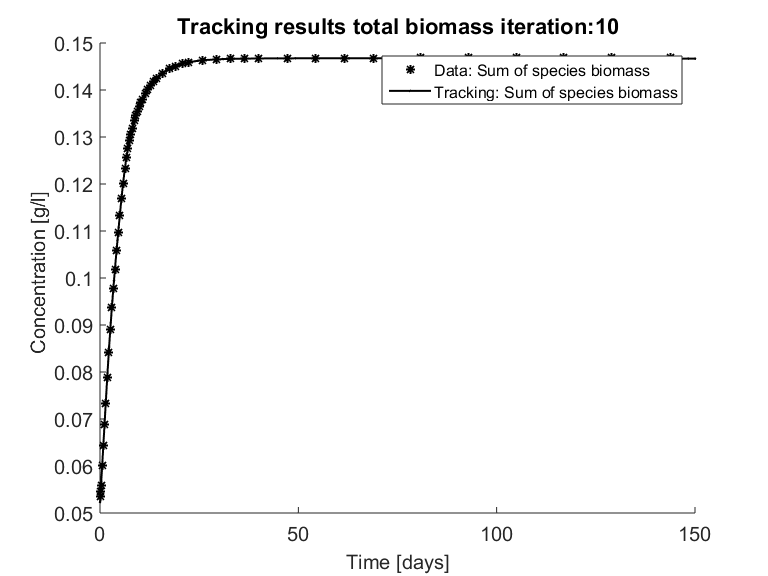
\includegraphics[width=0.5\textwidth]{Synthetic_data//lambda_=_e-1//191210_no_noise_Biomass_iter_10}
%	\caption{Total biomass. Dotted line: simulated data. Continuous line: the tracking procedure results.}
%	\label{Total Biomass no noise e1}
%\end{figure}
%\begin{figure}[h]
%	\centering
%	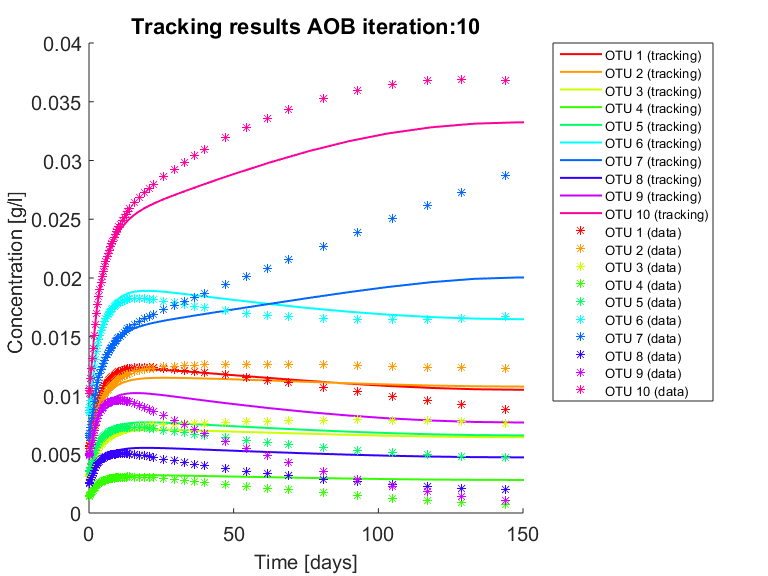
\includegraphics[width=0.5\textwidth]{Synthetic_data//lambda_=_e-1//191210_no_noise_AOB_iter_10_plot_1}
%	\caption{AOB biomass. Dotted line: simulated data. Continuous line: the tracking procedure results.}
%	\label{AOB no noise e1}
%\end{figure}
%\begin{figure}[h]
%	\centering
%	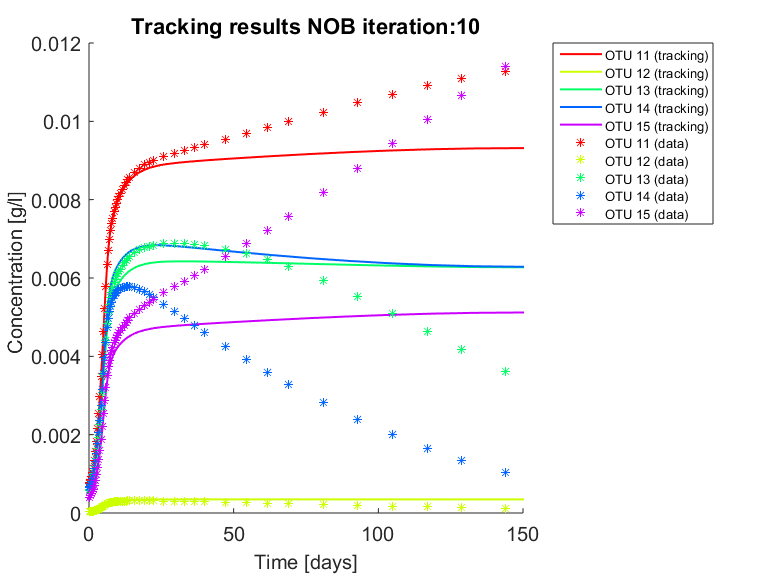
\includegraphics[width=0.5\textwidth]{Synthetic_data//lambda_=_e-1//191210_no_noise_NOB_iter_10_plot_1}
%	\caption{NOB biomass. Dotted line: simulated data. Continuous line: the tracking procedure results.}
%	\label{NOB no noise e1}
%\end{figure}
%\begin{figure}[h]
%	\centering
%	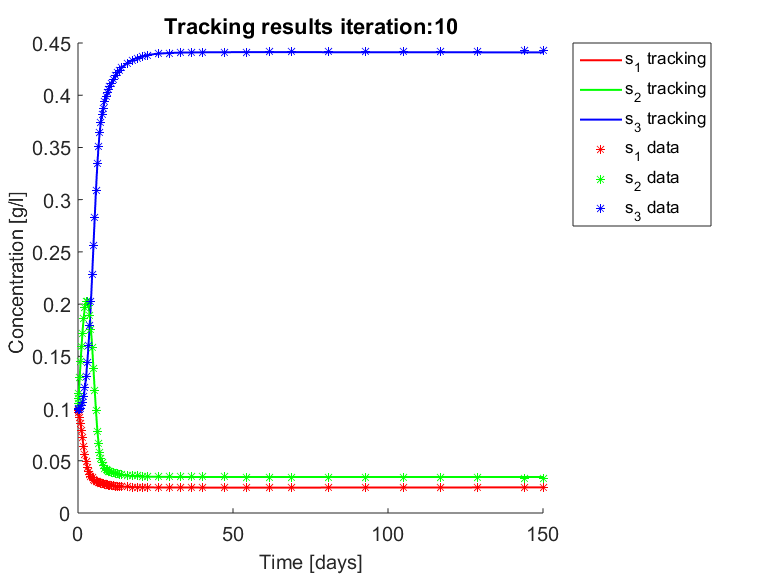
\includegraphics[width=0.5\textwidth]{Synthetic_data//lambda_=_e-1//191210_no_noise_metabolites_iter_10}
%	\caption{Metabolites. Dotted line: simulated data. Continuous line: the tracking procedure results.}
%	\label{Metabolites no noise e1}
%\end{figure}
%
%\begin{figure}[h]
%	\centering
%	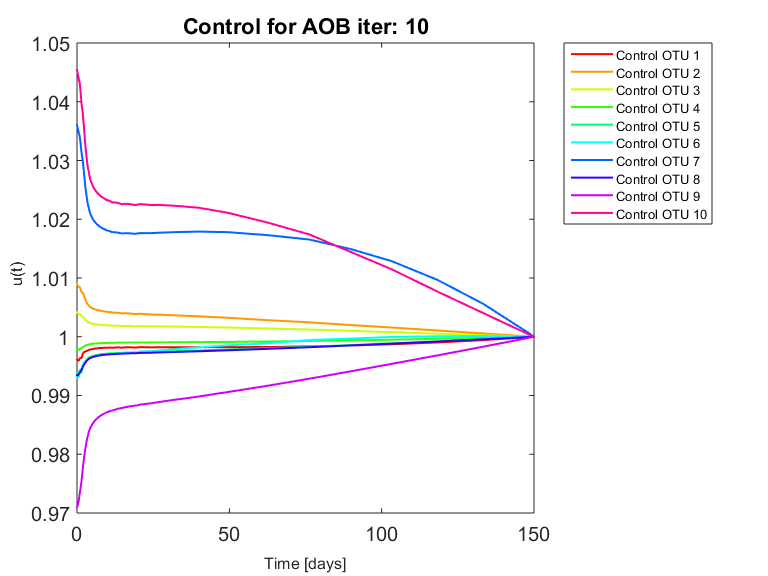
\includegraphics[width=0.5\textwidth]{Synthetic_data//lambda_=_e-1//191210_no_noise_Control_AOB_iter_10_plot_1}
%	\caption{Control for the AOB population.}
%	\label{Control AOB no noise e1}
%\end{figure}
%
%\begin{figure}[h]
%	\centering
%	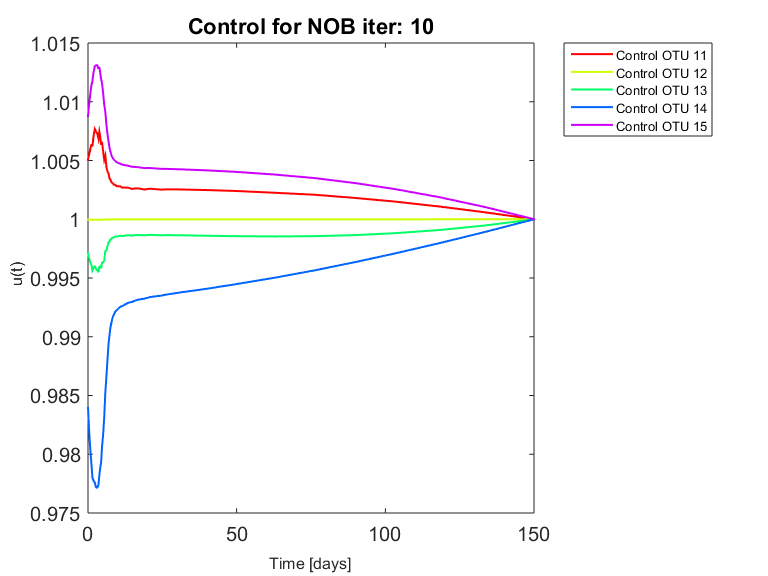
\includegraphics[width=0.5\textwidth]{Synthetic_data//lambda_=_e-1//191210_no_noise_Control_NOB_iter_10_plot_1}
%	\caption{Control for the NOB population.}
%	\label{Control NOB no noise e1}
%\end{figure}
%\clearpage
%\textbf{$\lambda = 10^{-2}$}
%\begin{figure}[h]
%	\centering
%	\includegraphics[width=0.5\textwidth]{Synthetic_data//lambda_=_e-2//191210_no_noise_2_Biomass_iter_10}
%	\caption{Total biomass. Dotted line: simulated data. Continuous line: the tracking procedure results.}
%	\label{Total Biomass no noise e2}
%\end{figure}
%\begin{figure}[h]
%	\centering
%	\includegraphics[width=0.5\textwidth]{Synthetic_data//lambda_=_e-2//191210_no_noise_2_Control_AOB_iter_10_plot_1}
%	\caption{AOB biomass. Dotted line: simulated data. Continuous line: the tracking procedure results.}
%	\label{AOB no noise e2}
%\end{figure}
%\begin{figure}[h]
%	\centering
%	\includegraphics[width=0.5\textwidth]{Synthetic_data//lambda_=_e-2//191210_no_noise_2_Control_NOB_iter_10_plot_1}
%	\caption{NOB biomass. Dotted line: simulated data. Continuous line: the tracking procedure results.}
%	\label{NOB no noise e2}
%\end{figure}
%\begin{figure}[h]
%	\centering
%	\includegraphics[width=0.5\textwidth]{Synthetic_data//lambda_=_e-2//191210_no_noise_2_metabolites_iter_10}
%	\caption{Metabolites. Dotted line: simulated data. Continuous line: the tracking procedure results.}
%	\label{Metabolites no noise e2}
%\end{figure}
%
%\begin{figure}[h]
%	\centering
%	\includegraphics[width=0.5\textwidth]{Synthetic_data//lambda_=_e-2//191210_no_noise_2_AOB_iter_10_plot_1}
%	\caption{Control for the AOB population.}
%	\label{Control AOB no noise e2}
%\end{figure}
%
%\begin{figure}[h]
%	\centering
%	\includegraphics[width=0.5\textwidth]{Synthetic_data//lambda_=_e-2//191210_no_noise_2_NOB_iter_10_plot_1}
%	\caption{Control for the NOB population.}
%	\label{Control NOB no noise e2}
%\end{figure}
%
%\clearpage

\bibliographystyle{elsarticle-num}
\bibliography{mybibfile}
\end{document}